\documentclass[10pt]{IEEEtran}
\usepackage{setspace}
\usepackage{psfig}
\usepackage{boxedminipage}
\usepackage{multirow}
\usepackage{amsmath}
\usepackage{cite}
\usepackage{times}
\usepackage[pdftex]{graphicx}
\usepackage{comment}
\usepackage{subfigure}
\usepackage{wrapfig}
% \usepackage{amsthm}
% \usepackage{enumerate}
\usepackage{multirow}

\begin{document}

\title{Bandwidth-Aware Reconfigurable Memory Design with Hybrid Memory
  Technologies}

% \author{\\
% \{\}@psu.edu\vspace{-10pt}
% }

\maketitle

\begin{abstract}
  In future chip-multiprocessor~(CMP) design, memory bandwidth is a potential
  bottleneck to system performance. Emerging non-volatile memory technologies,
  such as spin-torque-transfer memory~(STT-RAM), resistive memory~(RRAM), and
  embedded DRAM~(eDRAM), are promising solutions as on-chip memories for CMPs.
  In this paper, we propose a bandwidth-aware reconfigurable on-chip
  memory~(BAROM) design with hybrid memory technologies. We demonstrate a method
  to dynamically reconfigure the number of shared memory levels and capacity of
  each level based on statistical prediction. With a set of both multithreaded
  and multiprogrammed applications, we evaluate system performance obtained with
  our method. The experimental results show that the proposed reconfigurable
  hybrid memory design improves the overall system throughput by \% compared to
  pure SRAM memory design. In addition, our design leads to \% throughput
  increase and \% dynamic power reduction compared to hybrid but fixed memory
  hierarchy design.

\end{abstract}

% ------------------------------------------------------------------------------

\section{Introduction}

One potential bottleneck for chip-multiprocessor~(CMP) performance scaling is
the widening gap between the bandwidth demand created by processor cores and the
limited access bandwidth provided by off-chip main memory [15][16][6][20]. Such
limitation greatly affects the parallelism of memory demanding applications,
i.e., applications with a large working set, by consuming additional cycles on
off-chip memory access. In addition, even moderate memory demand applications
will be affected as the number of cores scales up [17]. The continuing shrink of
transistor density not only leads to increasingly powerful processors with a
large number of cores, but also puts much bandwidth pressure to off-chip main
memory. However, the bandwidth to the off-chip main memory does not improve much
compared to the processor core scaling. Potentially, these issues make the
applications running on the computing systems be bandwidth-bound at main memory.

While a number techniques can be found in today's systems and research work to
alleviate such bandwidth bottleneck, few can improve the system throughput in a
power and cost efficient manner. High performance computing machines such as
NVIDIA's Tesla~\cite{nvidia:tesla} rely on very high main memory bandwidths
(provided by GDDR memories) to feed the requirement from the processor. However,
GDDR memories run at higher clock rates and are more power hungry than
conventional DRAM modules. It is undesirable for either general purpose or high
performance computing systems to improve their computing performance by
sacrifacing power efficiency. With the emerging 3D chip technology, caches can
be stacked on top of processor cores to provide high memory
bandwidth[12][21][22]. However, ...

Caching has long been employed as the most effective approach to reduce memory
access latency. Adding an extra level of cache, however, can also help alleviate
the increasing bandwidth pressure of off-chip memory. In [dac.1] the authors
discuss extensively the problem of limited pin bandwidth to multiprocessor
systems. They have focused on program performance in multiprocessor systems and
make detailed decomposition of program execution times. They conclude that even
more complex on-chip cache structures would prove to be costeffective, with the
limited pin bandwidth severely restricting performance increases. In [dac.2] the
authors have carefully studied the requirements for on-chip cache structures
along with all sorts of optimization techniques that come along with scaling of
processor core numbers. Their study shows that cache size need to grow much
faster than processor core numbers to compensate for the limited off-chip
bandwidth. Because of that, the near future processors need to allocate a huge
percentage of chip area for caches, which means much less core counts than
expected. The study also shows that effective bandwidth optimization techniques
can help reduce cache size requirement and thus help scaling processor cores.
However, the effectiveness of caching in the mid/large scale multiprocessor
systems could be highly suboptimal due to significant contention across the
parallel tasks. The more bandwidth requirement by a workload can be satisfied by
the last level cache~(LLC), the less bandwidth will be required from the
off-chip main memory. Our memory technology pre-exploration shows that the
bandwidth provided by a memory decreases with the increase of its capacity.
Based on these observations, adding more levels of cache can potentially fill in
the bandwidth gap.

On-chip caches with fast random access, high storage density, and non-volatility
become possible due to the emergence of various new non-volatile memory~(NVM)
technologies, such as spin-torque-transfer memory~(STT-RAM), phase-change
memory~(PCRAM), and resistive memory~(RRAM). These emerging memory technologies
are believed to be promising solution as on-chip
caches~\cite{Sun:2009:MRAM-L2-CMP}. In addition to the benefit of
non-volatility, we demonstrate that these memory technologies provide higher
bandwidth than SRAM at a high capacity. Consequently, it is beneficial to use
NVM as lower level caches when large capacity.

This paper presents a bandwidth-aware memory hierarchy design to enhance system
performance of CMPs. Our goal is to enhance the memory system from the bandwidth
point of view, by leveraging these emerging memory technologies in devising a
hybrid cache hierarchy. The contributions we present in this paper include:

\begin{itemize}
\item Bandwidth-aware hybrid on-chip memory hierarchy design.
\item Hardware support that enables prediction of cache performance on the
  different sized caches.
\item OS scheduler support to make use of the prediction capability and
  appropriately schedule applications on to core with suitable cache capacity.

\end{itemize}

% -----------------------------------------------------------------------------

\section{Related Work}

The bandwidth problem of multicore processors has drawn much attention recently.
Yu \emph{et al.} proposed a LLC partitioning algorithm to minimize bandwidth
requirement to off-chip main memory~\cite{Yu:2010:OCMB}. While most cache
partitioning techniques focus on cache miss rates, our work takes a different
approach in which tasks�� memory bandwidth requirements are taken into account
when identifying a cache partitioning for multi-programmed and/or multithreaded
workloads. Cache resources are allocated with the objective that the overall
system bandwidth requirement is minimized for the target workload. The key
insight is that cache miss-rate information may severely misrepresent the actual
bandwidth demand of the task, which ultimately determines the overall system
performance and power consumption. <the moguls paper, the figure 1, however design for
induvidual application, i.e., with different application can generate different
designs.>

A large body of recent research focuses on exploring new memory technologies to
trade off between latency, bandwidth, and cost. Wu et al. explored various
memory technologies - SRAM, eDRAM [23], magnetic RAM (MRAM) [12] and PCM to best
construct L3 caches in terms of performance and power [24]. The eDRAM and MRAM
technologies are evaluated as LLCs by stacking each memory on top of the
processor die. Both studies mainly focused on reducing the latency gap between L2
cache~(LLC) and external memory and do not examine the bandwidth. <nvm cache
research: most for latency, not bandwidth opt.>


Application behavior prediction is a critical component of reconfigurable
architectures. Zhou \emph{et al.} monitored memory access patterns and estimated
memory behavior of workloads for energy efficient memory allocation
[predictor.26]. Duesterwald et al. [10] describe different statistical and table
based predictors for within- and across-metric predictions of performance
monitoring information. They show that the table-based predictor generally
outperforms the other predictors they tested. Sarikaya et al. [19] describe an
optimal prediction technique based on a predictive least squares minimization.
Sarikaya \emph{et al.} showed the benefit of statistical metric modeling for
tracking varying pattern history lengths and modeling long term
patterns~\cite{Sarikaya:2011:RWBP}. However, ...

% -----------------------------------------------------------------------------

\section{Background}

\noindent{}{\bf{STT-RAM}} STT-RAM uses the magnetic property of the material and
uses Magnetic Tunnel Junction (MTJ) as its binary storage. As shown in
Fig.~\ref{fig:mram_cell}, MTJ contains two ferromagnetic layers and one tunnel
barrier layer. The direction of one ferromagnetic layer is fixed, which is
called the reference layer, while the direction of the other one can be changed
by passing a driving current, which is called the free layer. The relative
magnetization direction of two ferromagnetic layers determines the resistance of
MTJ. If two ferromagnetic layers have the same directions, the resistance of MTJ
is low, indicating a ``0'' state; if two layers have different directions, the
resistance of MTJ is high, indicating a ``1'' state. \vspace{0.1in}

\begin{figure}[t]
\centering
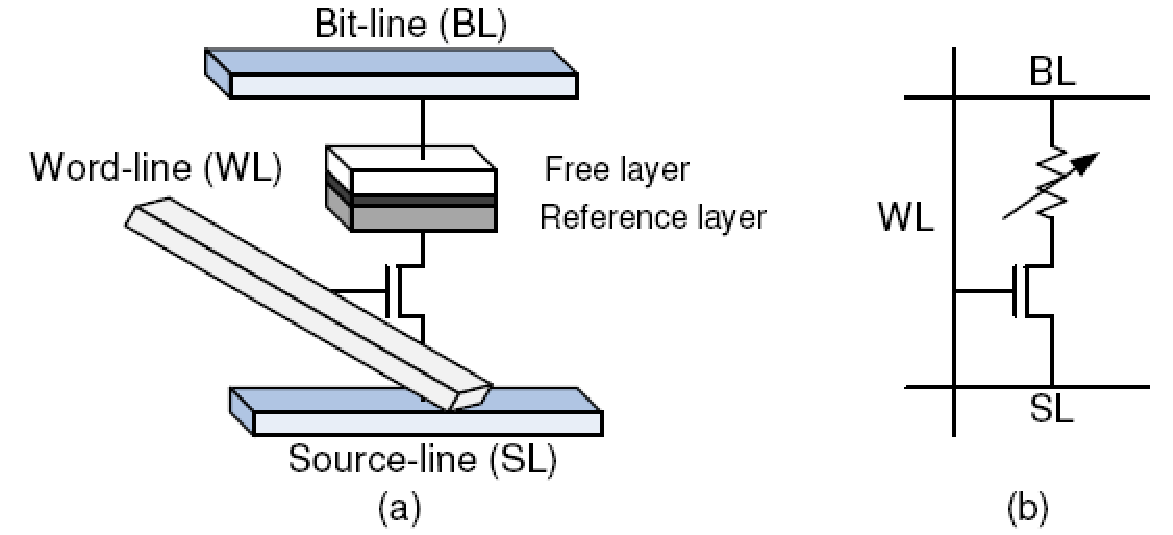
\includegraphics[width=2.5in]{figures/mram_cell}
\caption{Demonstration of a MRAM cell. (a) Structural view. (b) Schematic view.}
\label{fig:mram_cell}
\end{figure}

% \noindent{}{\bf{PCRAM}} PCRAM uses chalcogenide-based material to storage
% informations. The chalcogenide-based materials in recent PCRAM research are
% usually alloys of germanium, antimony, and tellurium (GeSbTe, or GST), which can
% be switched between a crystalline phase (SET or ``1'' state) and an amorphous
% phase (RESET or ``0'' state) with the application of heat. The crystalline phase
% shows high optical reflectivity and low electrical resistivity, while the
% amorphous phase is characterized by low reflectivity and high resistivity.

% \begin{figure}[t]
% \centering
% 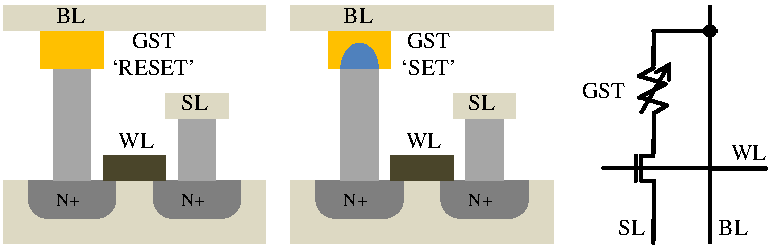
\includegraphics[width=2.5in]{figures/GST}
% \caption{The schematic view of a PCRAM cell with MOSFET selector transistor (BL=Bitline, WL=Wordline, SL=Sourceline}
% \label{fig:GST}
% \end{figure}

\noindent{}{\bf{RRAM}} Memristor, a portmanteau of ``memory resistor'', is a
generalized resistance that maintains a functional relationship between the time
integrals of current and voltage. Memristor was first theoretically predicted by
Chua in 1971~\cite{memristor:chua} as the fourth fundamental circuit element
from the completeness of relations between the four basic circuit variables,
namely, current, voltage, charge, and flux-linkage. The first memristor
practical demonstration was presented by Williams \emph{et al.} in
2008~\cite{memristor:missing}. Fig.~\ref{fig:memristor} shows a conceptual view
of the memristor structure~\cite{memristor:missing}. The top electrode and
bottom electrode are two metal nanowires on platinum, and the thin titanium
dioxide film is sandwiched by the electrodes.

\begin{figure}[t]
\centering
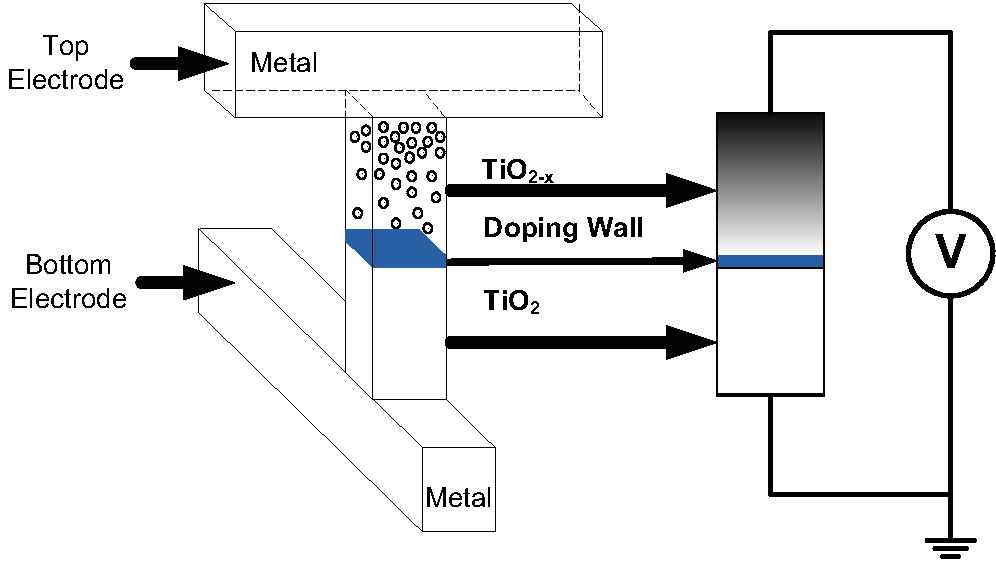
\includegraphics[width=2.5in]{figures/memristor}
\caption{The conceptual view of the structure of memristor cells.}
\label{fig:memristor}
\end{figure}

\noindent{}{\bf{eDRAM??}}

% -----------------------------------------------------------------------------
\section{Memory Technology Exploration}
Many modeling tools have been developed during the last decade to enable
system-level design exploration for SRAM- or DRAM-based cache and memory design.
For example, CACTI~\cite{CACTI} is a tool that has been widely used in the
computer architecture community to estimate the speed, power, and area of SRAM
and DRAM caches. In addition, CACTI has also been extended to evaluate the
performance, power, and area for STT-RAM~\cite{CACTI:DAC08:Dong},
PCRAM~\cite{CACTI:GLSVLSI08:Mangalagiri,CACTI:PCRAMsim}, and NAND
flash~\cite{CACTI:DATE10:Mohan}. However, as CACTI is originally designed to
model SRAM-based cache, some of its fundamental assumptions do not match the
actual NVM circuit implementation, and thereby these CACTI-like estimation tools
do not model the NVM array organization in the exact way that the chip is
fabricated. In this section, we use \emph{NVSim}, a circuit-level model for NVM
performance, energy, and area estimation, which supports various NVM
technologies including STT-RAM, PCRAM, RRAM, and conventional NAND flash.

\begin{figure*}[t]
\centering
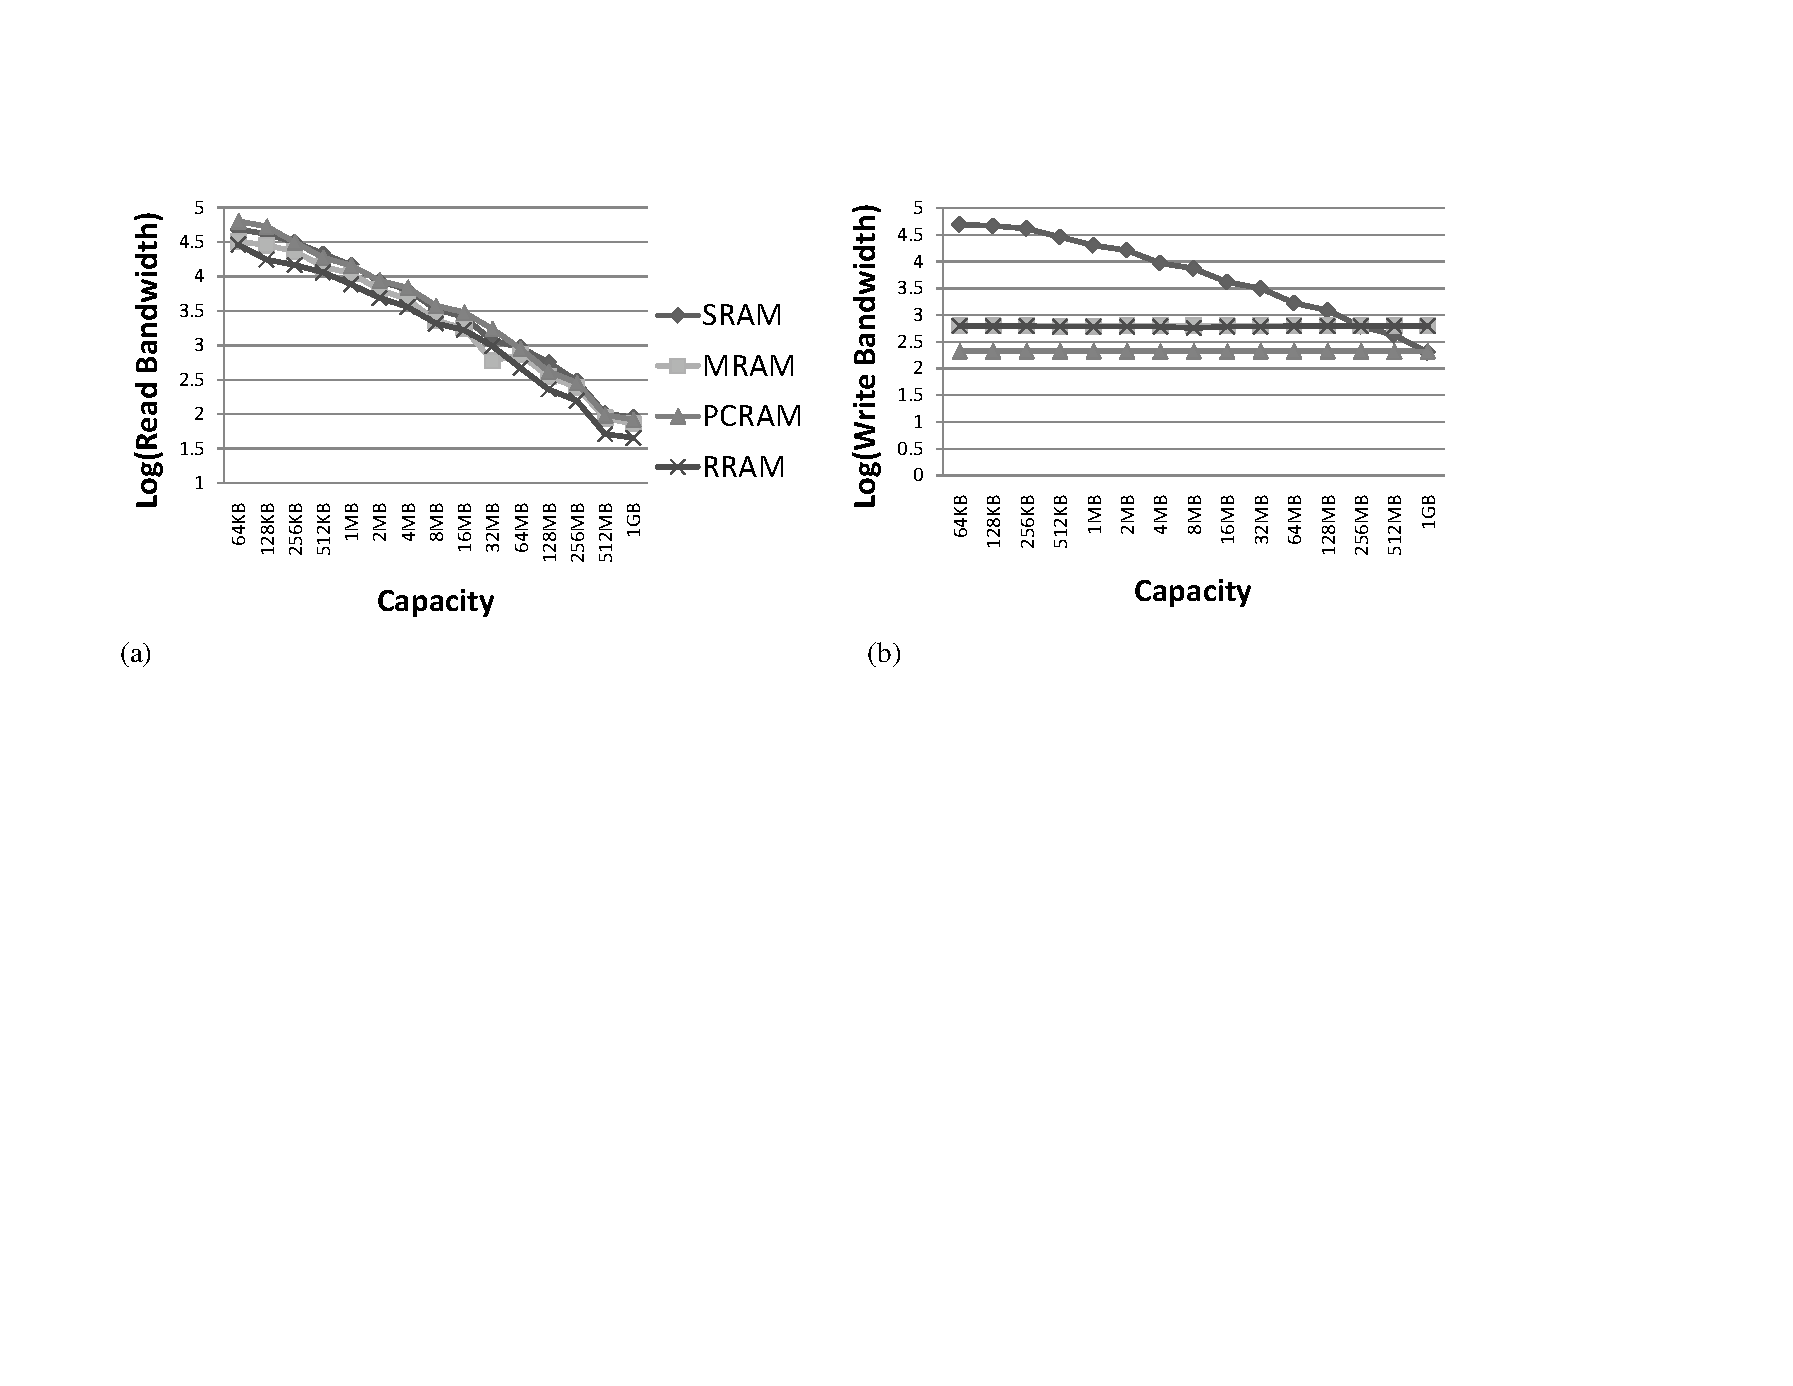
\includegraphics[width=5in]{figures/RAM_bandwidth}
\caption{Read and write bandwidths provided by different memory technologies.
(a) Read bandwidth provided by different memory technologes. (b) Write bandwidth
provided by different memory technologies.}
\label{fig:memory-bw}
\end{figure*}

First of all, we estimate the read and write bandwidths that can be provided by
different memory technologies. Figure~\ref{fig:memory-bw} shows the results,
with both x- and y-values in \emph{log} scale. The figure illustrates both the
provided read and write bandwidth as a function of memory capacity. Each of the
memory technologies actually provide nearly the same read bandwidths, as is
shown in figure~\ref{fig:memory-bw}(a). On the other hand, a straight forward
observation from figure~\ref{fig:memory-bw}(b) is that the write bandwidth
varies among different memory technologies. The shape of the SRAM write
bandwidth curve is very similar to the read bandwidth curve. The write bandwidth
curves of the other three memory technologies appear to be very different. The
reason is that write latencies of the three non-volatile memories are much
higher than read latencies. Another observation from
figure~\ref{fig:memory-bw}(b) is that the curves cross to each other at
different locations.

\begin{figure*}[t]
\centering
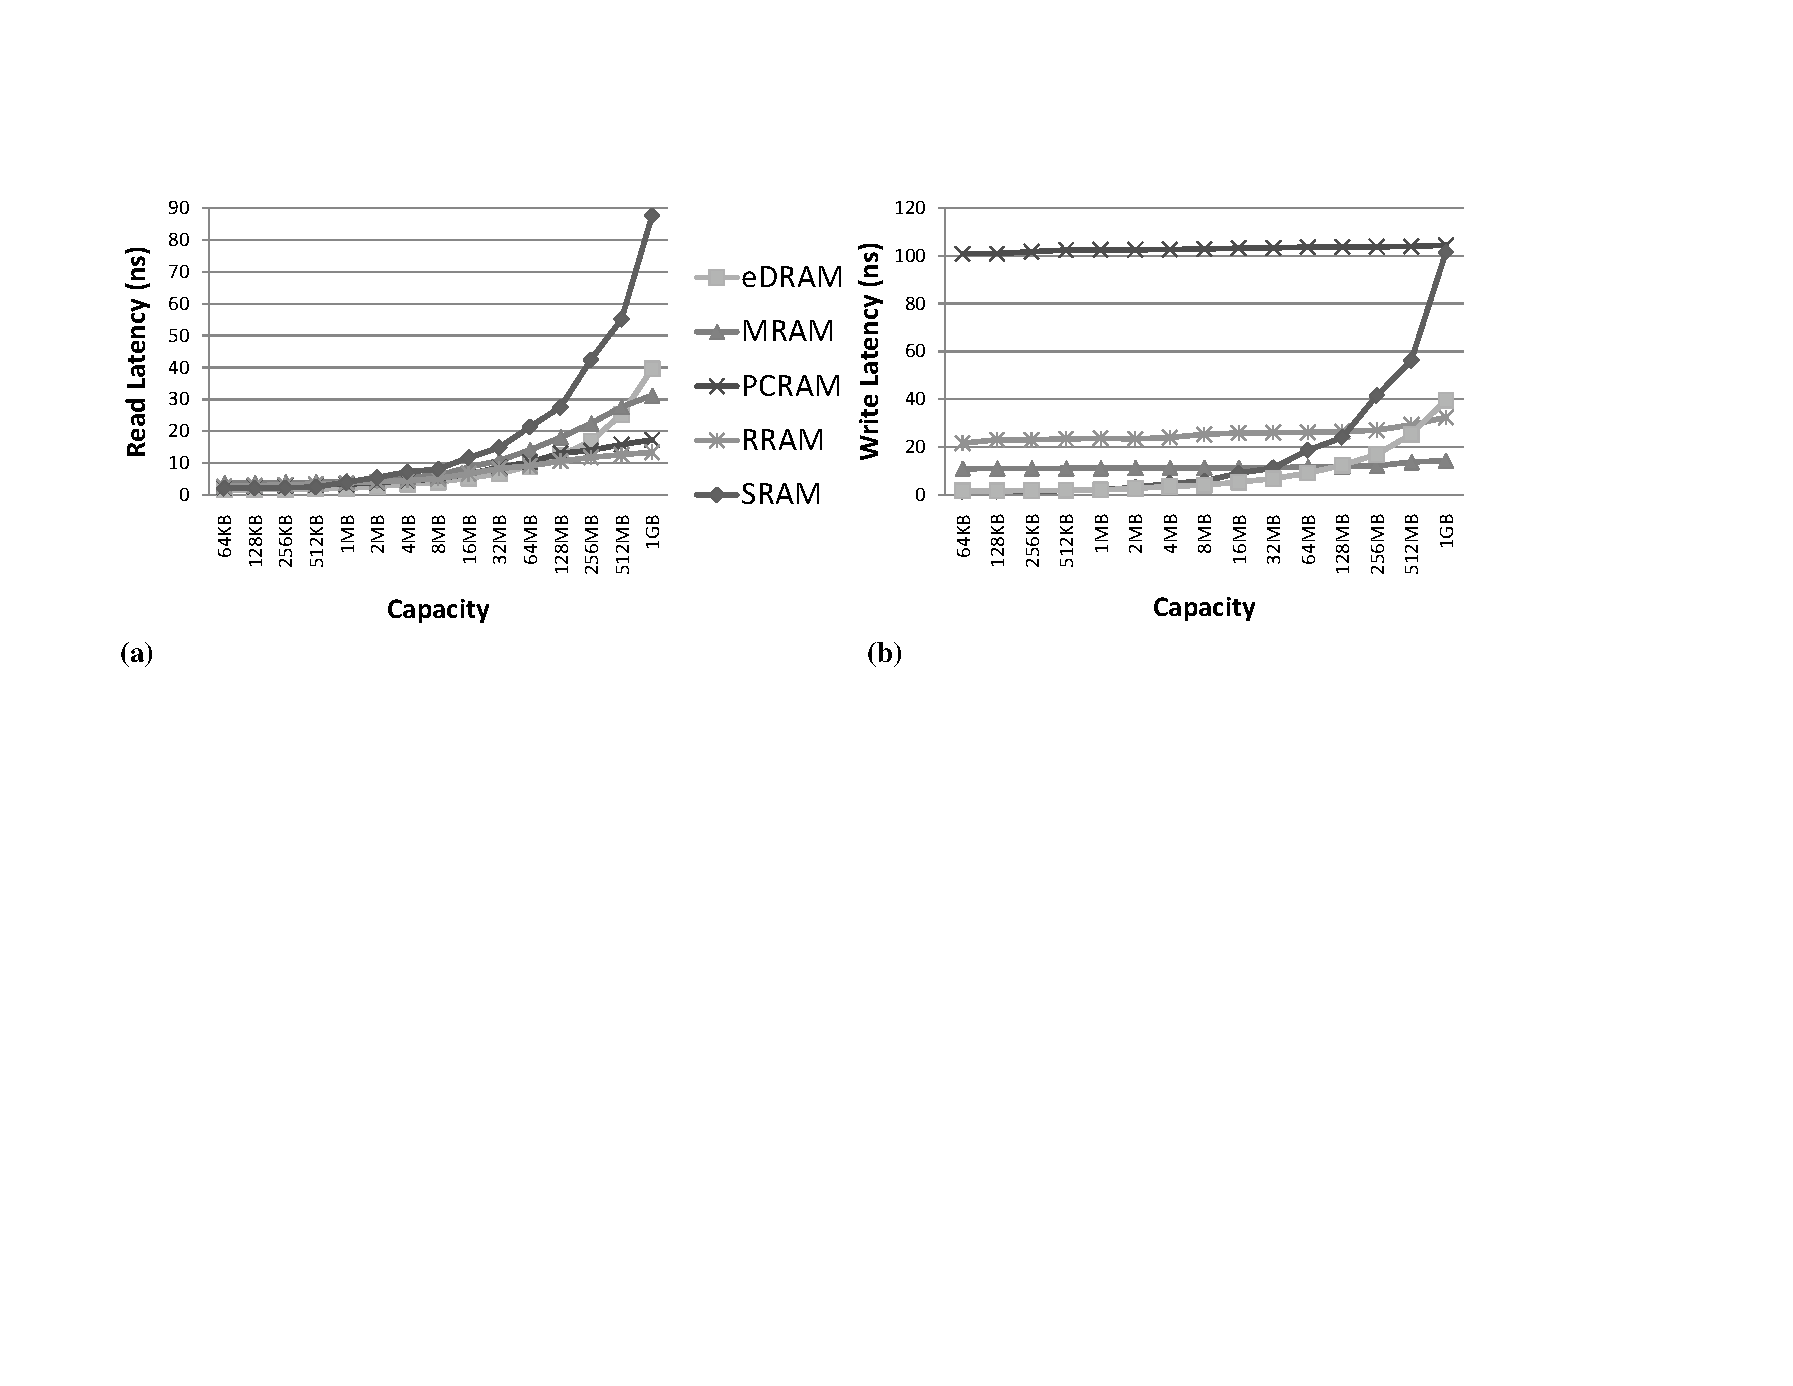
\includegraphics[width=5in]{figures/RAM_latency}
\caption{Latency of different memory technologies. (a) Read Latency. (b) Write Latency.}
\label{fig:memory-latency}
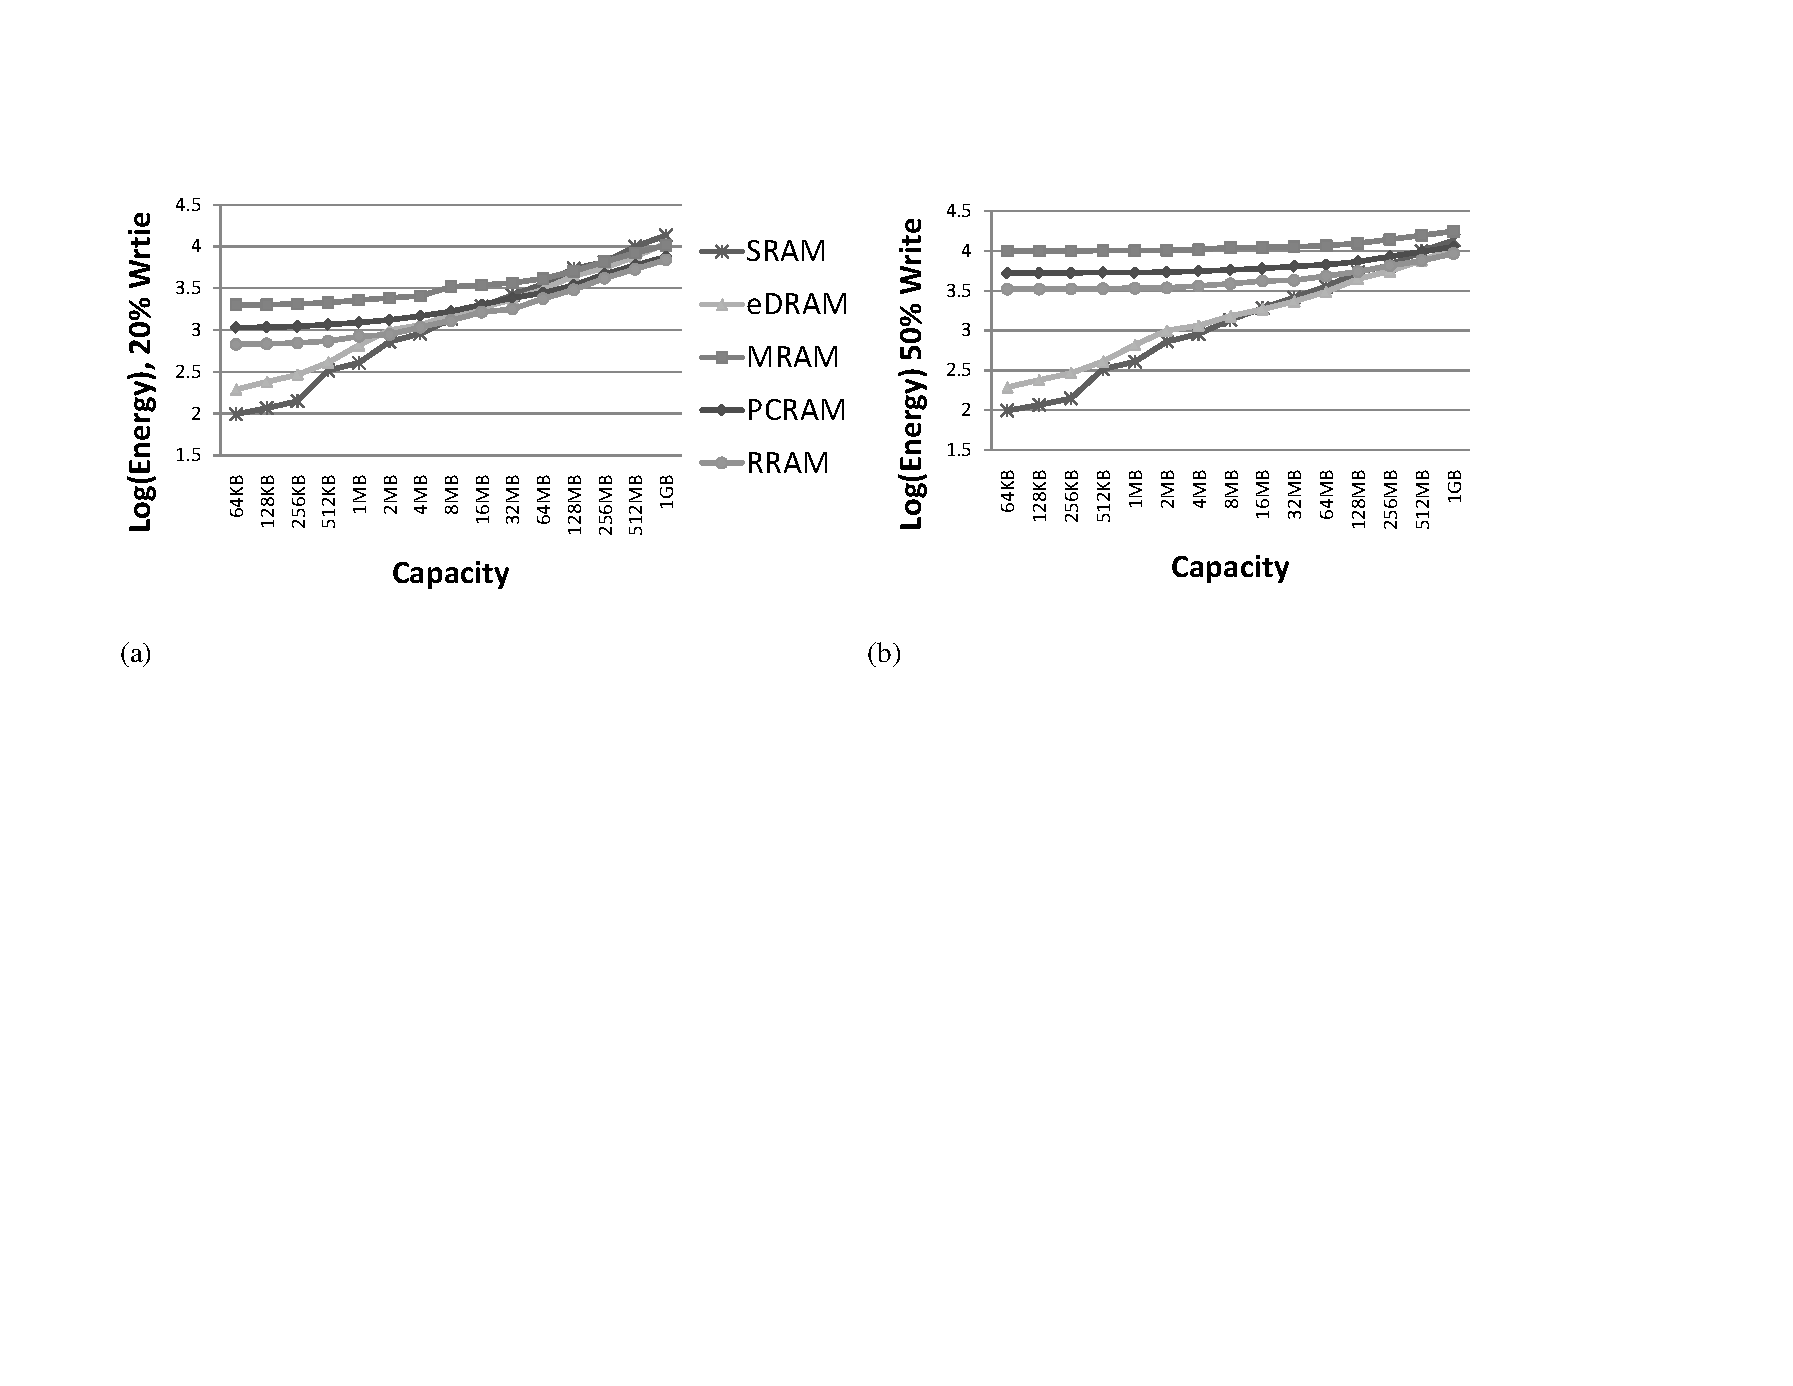
\includegraphics[width=5in]{figures/RAM_energy}
\caption{Dynamic energy consumption with the provided bandwidths of different
  memory technologies. (a) Dynamic Energy with 20\% write.  (b) Dynamic Energy with 50\% write. }
\label{fig:memory-energy}
\end{figure*}

Being aware that the read and write latencies of NVM are asymmetric, we consider
the read latency at first. In NVsim, we divide the entire cache read latency
into the following components:
\begin{enumerate}
\item H-tree input delay
\item Decoder + word-line delay
\item Bit-line delay + Sense Amplifier delay
\item Comparator Delay (for tag part only)
\item H-tree output delay
\end{enumerate}
H-tree latencies 1) and 5) are mainly determined by the RC delay of global
wires, which is positive proportional to the area of memory macro. Sensing delay
4) is related to the read noise margin of memory cell that is affected by off/on
resistance ratio. Figure~\ref{fig:memory-latency} (a) illustrates the read
latency of different memories. We can see that sensing delay dominates the read
latency of NVM at small capacity so that PCRAM (with the largest resistance
window) is faster than RRAM and MRAM (with the smallest resistance window).
While H-tree delay unveils at large capacity so that RRAM (with the smallest
cell size) becomes faster than PRAM and MRAM (with the biggest cell size). The
read latency of SRAM bank will increase rapidly after 128MB due to large area.

Write latency of NVM are almost dominated by the write pulse width. In this work
we assume 10ns, 20ns, 100ns for MRAM, RRAM and PCRAM. While write latency of
SRAM and eDRAM is a function of capacity, as similar to the read latency. The
results in ~\ref{fig:memory-latency} (b) indicates that NVM is suitable for
memory with large capacity.

Figure~\ref{fig:memory-energy} has demonstrated the dynamic energy of different
memory technologies when 20\% and 50\% write access are assumed. eDRAM will be
better than SRAM in terms of dynamic energy after 16MB and this is verified by
IBM Power7 L3 cache. The cross-point between NVM and SRAM/eDRAM is postponed for
50\% write than 20\% write.

Based on these observations, we would like to design a bandwidth-aware hybrid
memory hierarchy, which always provides the high memory bandwidth with the given
capacity. For example,
\begin{itemize}
\item eDRAM has better latency and enegry than SRAM when capacity is larger than
  16MB.
\item MRAM is more competitive to SRAM and eDRAM when capacity is larger than
  128MB.
\item PCRAM has serious endurance issue and is targeted as main memory
  replacement.
\item RRAM might fit into cache hierarchy as last level cache replacement when
  there multiple levels of cache for applications with very few writes.
\end{itemize}

% -------------------------------------------------------------------------
\section{Design Method}

Based on our memory technology exploration, we now provide an overview of BAROM
design. While many design methods envolved with new memory technologies endeavor
to reduce the off-chip memory access latency, this work focuses on minimize
off-chip bandwidth requirement by employing hybrid on-chip memory and
reconfiguration. For each level of memory, we select the memory technology that
has the highest provided bandwidth within given capacity. On top of such
hardware hierarchy design, we apply dynamic memory system reconfiguration with
the bandwidth demand of a specific set of applications as the major metric. One
desirable characteristic of BAROM is that it provides prioritized access to the
residual memory capacity available at runtime instead of sharing it among all
data flows. By having control over the residual capacity, we can better utilize
the limited resources to enhance system performance. The hardware
reconfiguration is further facilitated by software prediction engine. Rather
than conventional last value predictors and table-based predictors, we employ a
probablity-based predictor that can achieve higher accuracy with small
performance overhead. The rest of this section describes the BAROM design, which
is composed of on-chip memory hierarchy hardware design, the reconfiguration
mechanism, and the predictor engine.

\subsection{Hardware Configuration}

Figure~\ref{fig:hw-config} shows an overview of BAROM hardware configuration.
The CMP system consists of multiple cores, where L1 cahces are private to each
core and lower level caches are shared by the cores. With the provided bandwidth
vs. capacity curves of various memory technologies that are obtained using the
method described in section~\ref{sec:tech-explore}, we can design a hybrid
on-chip memory system to always provide the highest bandwith. In order to
achieve this goal, we configure the memory hierarchy in the following
manner.\vspace{5pt}

\noindent{}{\bf{Number of levels.}} In order to decide the number of memory
levels, we examine the provided bandwidth curve. Memory levels are seperated by
the cross points of two memory technologies. For example,
Figure~\ref{fig:memory-bw} illustrates that there are two cross points (SRAM and
STT-RAM, STT-RAM and RRAM). Therefore, we will have three levels of shared
caches.\vspace{5pt}

\noindent{}{\bf{Memory technology of each level.}} The memory technology with
the highest provided bandwidth within the given range of capacity of each level
is selected. In our case, SRAM, STT-RAM, and RRAM are selected as the L2, L3,
and L4 caches respectively. \vspace{5pt}

\noindent{}{\bf{Capacity of each level.}} The maximum availabe capacity of each
level is determined by the cross point of two memory technologies. In our case,
the capacities of SRAM/L2, STT-RAM/L2, and RRAM/L4 are 2MB, 512MB, and 1GB
respectively. At the system initialization, the capacity of each level is
defined to be the maximum available capacity of the level. According to the
reqirement of different applications, the capacities can be reconfigured at
run-time to provide best performance. The memory space of each level can also be
reconfigured to form an internal level as shown in Figure~\ref{fig:hw-config}.
The hardware and software supports for reconfiguration will be presented in the
following sections.\vspace{5pt}

The goal of such architecture design is to make use of different memory
technologies to configure an on-chip memory system with optimal provided
bandwidth over a range of capacities. As a result, the overall provided
bandwidth curve of the on-chip memory system will appear to be an envelope line
of all the available memory technologies as illustrated in
Figure~\ref{fig:pbw-envelope}. It is illustrated in this figure that the hybrid
memory system always provides the highest bandwidth over different capacities.

\subsection{Reconfiguration}

Although the above hybrid memory configuration maintains the optimal provided
bandwidth curve over all the capacities, it does not garantee the best
performance for different applications with a variety of bandwidth requirements.
The overall provided bandwidth curve shown in Figure~\ref{fig:pbs-envelope}
appears to be monotonically decreasing. A specific application may have a
bandwidth requirement that can be mapped to a single point on the curve. In
order to satisfy the bandwidth demand of different applications, we dynamically
reconfigure the memory space of each level corresponding to the bandwidth
requirement of each set of applications running on the system. To be more
aggressive, the reconfiguration is applied at the end of each given execution
time interval to accomodate different program phases of applications.

The major system parameter to be reconfigured is the capacity of each memory
level. At each time interval, we determine the upper bound of the capacity of
memory level-i ($s_{iu}$) by mapping the demand bandwidth (DBW) of a specific
application to the system's provided bandwidth curve, i.e.,
$s_{iu}=f^{-1}(\textrm{DBW})$ where $f(x)$ represents the provided bandwidth
curve of the on-chip memory system stored in the look-up-table in a reserved
non-volatile memory space. The demand bandwidth for each memory level is
generated using the prediction engine presented in section~\ref{sec:predict}. In
previous sections, we show that the memory with smaller capacity provides higher
bandwidth. Theoritically, the higher bandwidth provided by the memory system
leads to higher performance (in terms of throughput) and power consumption of
throughput computing applications~\cite{throughput-vs-bandwidth}. Consequently,
we define a lower bound of memory capacity as
$s_{il}=f^{-1}(\textrm{DBW}*(1+\sigma))$, where $\sigma$ is a pre-defined
threshold to make sure possible provided bandwidth increase without much power
overhead. The capacity of memory level-i ($s_i$) is therefore selected to
satisfy $s_{il}\le s_i\le s_{iu}$.

Our primary reconfigurable design exploits set associativity in conventional
cache organizations. Figure~\ref{fig:reconfig} depicts the block diagram for the
organization of our design. An n-way set associative cache consists of $n$ data
and tag arrays. We divide the each level of on-chip memory into partitions at
the granularity of the $k$-ways, where $k$ is determined by the number of
available capacity values for a specific memory technology on the provided
bandwidth curve. For example, if there are 8 available capacities for STT-RAM
(from 2MB to 1GB), we will determine the granularity by $k=n/8$.The desirability
of such configuration is to exploit the division of ways already present in a
conventional cache organization.


The index part of the input address is used to index all the
ways of the data and tag array. The tag part of the input address is sent to the
comparators of all the ways to determine if there is a match with any of the
tags read from the tag array. If there is a match, a hit is signaled on the
valid output line and data from the corresponding way of the data array is sent
onto the output data lines.
 







reconfiguration support: how reconfigurable (Li -> Li+1 (Li+0.5); hardware
modification to support reconfiguration.


reconfigure the unused capacity:

- if (> si): becomes si+1

- else: unused (or becomes lut)



\subsection{Prediction Engine}

statistical prediction

hierarchical prediction

performance opt: lut long enough but not too long (num of entries, bits per
entry)

% -------------------------------------------------------------------------
\section{Experiments}

Based on the parameters of different cache configurations collected from our
modified version of CACTI~\cite{CACTI}, we evaluate both pure SRAM-based and
hybrid cache hierarchy designs. In this section, we show how bandwidth-aware
memory hierarchy design method help with improving the system performance.

\subsection{Experimental Setup}

We use Simics~\cite{Magnusson:2002:simics-orig-paper} as the simulator in our
experiments. It is configured to model an eight-core CMP. Each core is in-order, and
is similar to UltraSPARC III architecture. The frequency of each core is set to
be 1GHz. Table~\ref{table:cmp-config} lists the detailed parameters of the
baseline. Our baseline contains 8 private L1 instruction and data caches
respectively. Since we only evaluate shared cache hierarchies, each of L1 cache
is fixed to be SRAM-based, and of 64KB capacity. As regard to lower level
caches, we evaluate two cases, pure SRAM-based and hybrid caches with various
memory technologies, including SRAM, MRAM, RRAM, and eDRAM. By evaluating both
cases, we would like to find out optimal cache design that leads to the peak
performance, i.e., the number of cache levels that is reqired, memory technology
used for each level, and capacity of each level.

\begin{table}[t]
  \centering
  \caption{Baseline CMP configuration.}
  \begin{tabular}{l|c}
    \hline\hline
    \multicolumn{2}{l}{\textbf{Core}}\\
    \hline
    No. of cores & 8\\
    \hline
    Frequency & 1GHz\\
    \hline
    Core architecture & in-order, 14-stage pipeline\\
    \hline
    \multicolumn{2}{l}{\textbf{Memory}}\\
    \hline
    \multirow{2}{*}{Private caches} & L1-I/D caches: SRAM, 8 x 64KB,\\
                                    & 64B line, 2-way, write-through \\                                    
    \hline
    \multirow{2}{*}{Shared caches} & Case 1: Pure SRAM, 64B line,\\
                                   & 8-way, write-back\\
                                   & Case 2: Hybrid~(SRAM, MRAM,\\
                                   & RRAM, eDRAM), 64B line,\\
                                   & 8-way, write-back\\
    \hline
    Main memory & 4GB\\
    \hline\hline
  \end{tabular}
  \label{table:cmp-config}
\end{table}

The benchmarks are selected from PARSEC benchmark suite~\cite{PARSEC:2008} with
multithreaded programs, which focus on emerging workloads that are designed to
be representative of next-generation shared-memory programs for CMPs. Since the
performance of different memory technologies are closely related to read and
write intensities, we selected some workloads that vary in the average numbers
of L2 cache read per thousand instructions~(RPKI) and write per thousand
instructions~(WPKI), which are listed in
Table~\ref{table:benchmarks}.

\begin{table}[t]
  \centering
  \caption{Characteristics of selected benchmarks.}
  \begin{tabular}{l|c|c}
    \hline\hline    
    \textbf{Benchmarks} & \textbf{RPKI} & \textbf{WPKI}\\
    \hline
    blackscholes & 22.8 & 61.7\\
    \hline
    bodytrack & 5.4 & 139.5\\
    \hline
    canneal & 5.4 & 29.3\\
    \hline
    facesim & 6.0 & 102.4\\ 
    \hline
    ferret & 5.7 & 173.4\\
    \hline
    fluidanimate & 2.6 & 70.1\\
    \hline
    streamcluster & 17.3 & 16.9\\
    \hline
    swaptions & 2.6 & 121.4\\
    \hline\hline
  \end{tabular}
  \label{table:benchmarks}
\end{table}

\subsection{Results}

We evaluate various possible configurations with shared caches by simulation,
i.e., with possible numbers of levels, memory technologies, and cache capacities
for each cache level. We consider SRAM and eDRAM as the possible memory
technologies to implement L2 and L3 caches. Both MRAM and RRAM have higher write
latency than SRAM. Furthermore, the endurance of RRAM is too low to be used as
lower level caches. Consequently, these two memory technologies are only
considered to be used as the last level cache.

In the first set of experiments, we evaluate the system performance with
two-level shared caches. Figure~\ref{fig:thput-l2l3} shows the system throughput
with all the benchmarks. It is illustrated that implementing hybrid cache with
eDRAM as the L3 cache helps with performance among most of the benchmarks. Such
performance improvement is more than 10\% in Figure~\ref{fig:thput-l2l3}(a). It
is indicated by our memory technology exploration that eDRAM shows more latency
benefits with larger capacities. As a result, a larger eDRAM-based L3 cache
leads to more performance improvement to the pure SRAM implementation, as
illustrated by Figure~\ref{fig:thput-l2l3}(b). However, hybrid cache does not
always improve the performance, as shown in Figure~\ref{fig:benchmark-l2l3}.
With the benchmark \emph{canneal}, hybrid cache configurations outperform the
pure SRAM implementation among overall range of various capacities. With the
benchmark \emph{ferret}, however, pure SRAM implementation results in higher
performance than hybrid cache implementation with the same capacity
configuration.

\begin{figure*}[t]
\centering
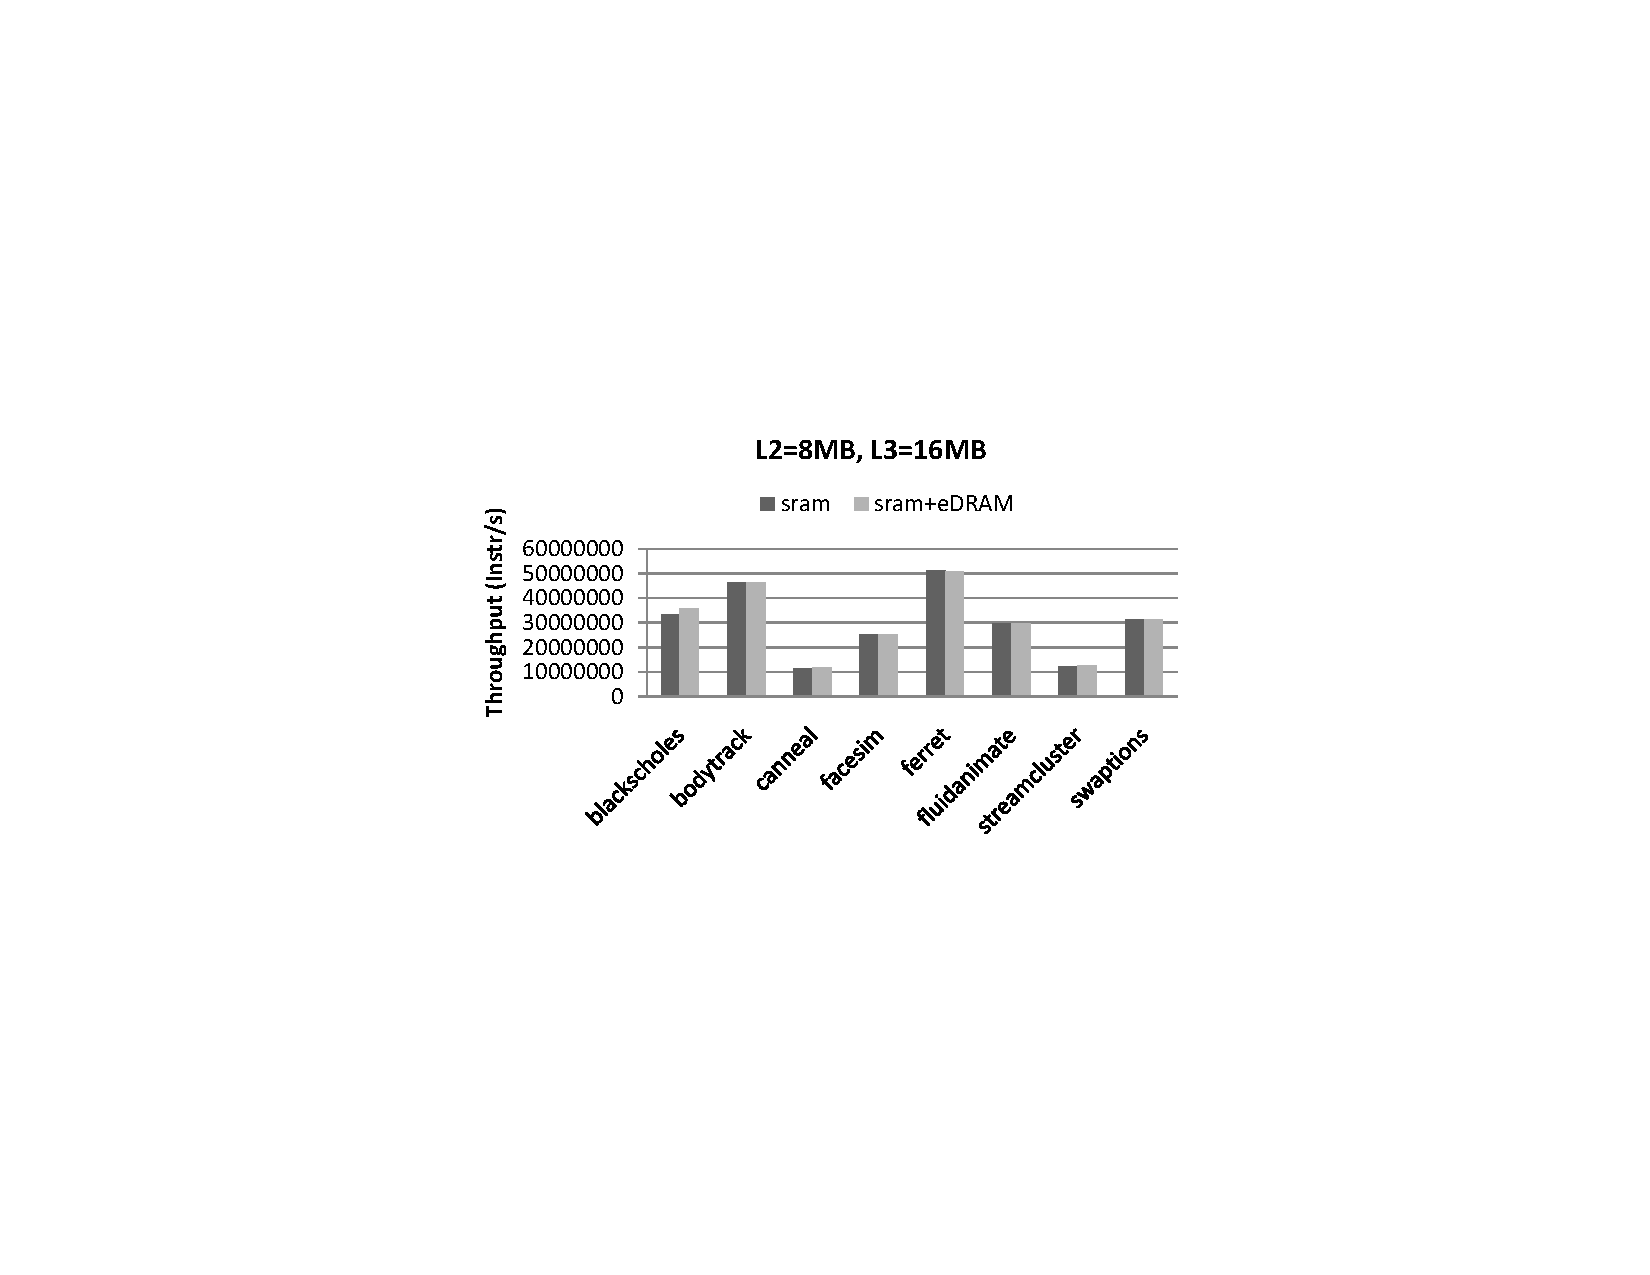
\includegraphics[width=2.5in]{figures/thput-l2l3-1}\hspace{0.2in}
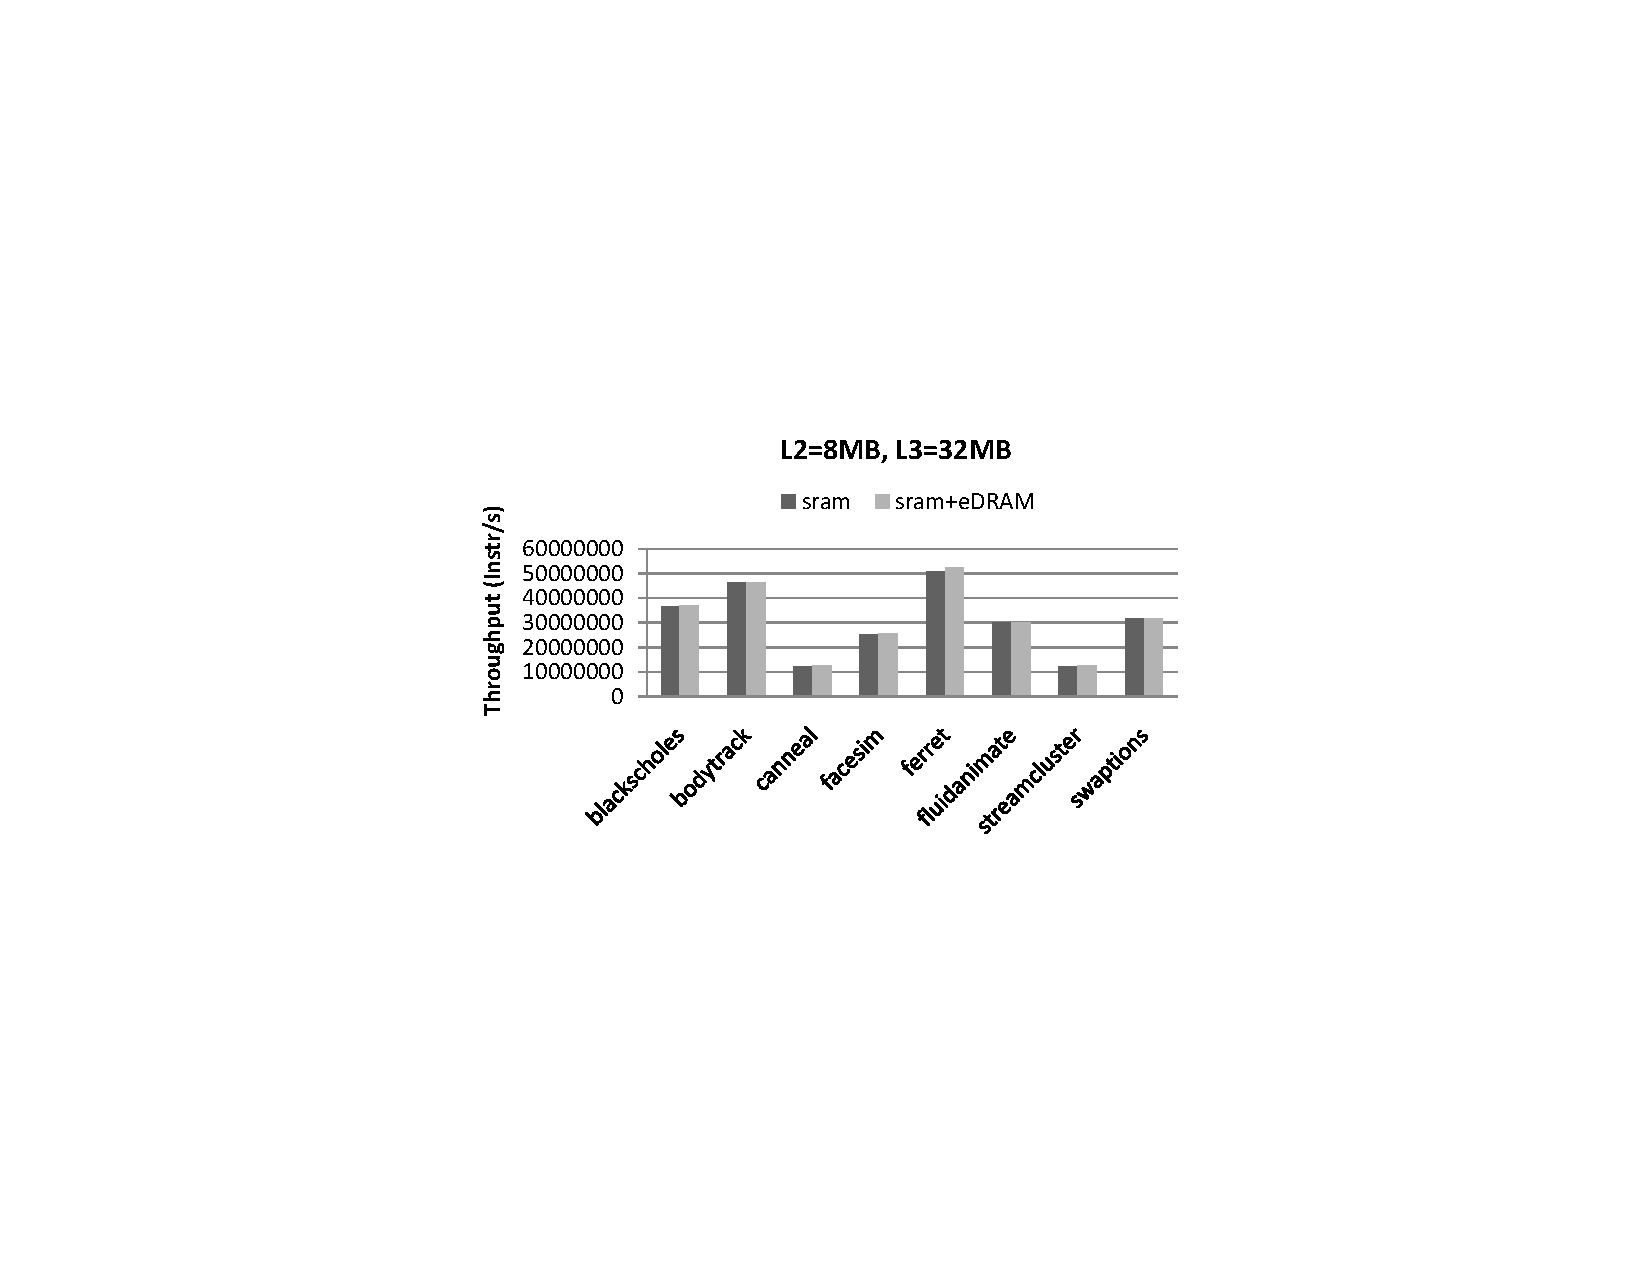
\includegraphics[width=2.5in]{figures/thput-l2l3-2}\\
\hspace{0.02in}
\makebox[2.5in][l]{\bf (a)}
\makebox[2.5in][l]{\bf (b)}
\caption{Performance comparison with two-level caches among various benchmarks.
  (a) The L3 cache capacity is 16MB. (b) The L3 cache capacity is 32MB.}
\label{fig:thput-l2l3}
\end{figure*}

\begin{figure*}[t]
\centering
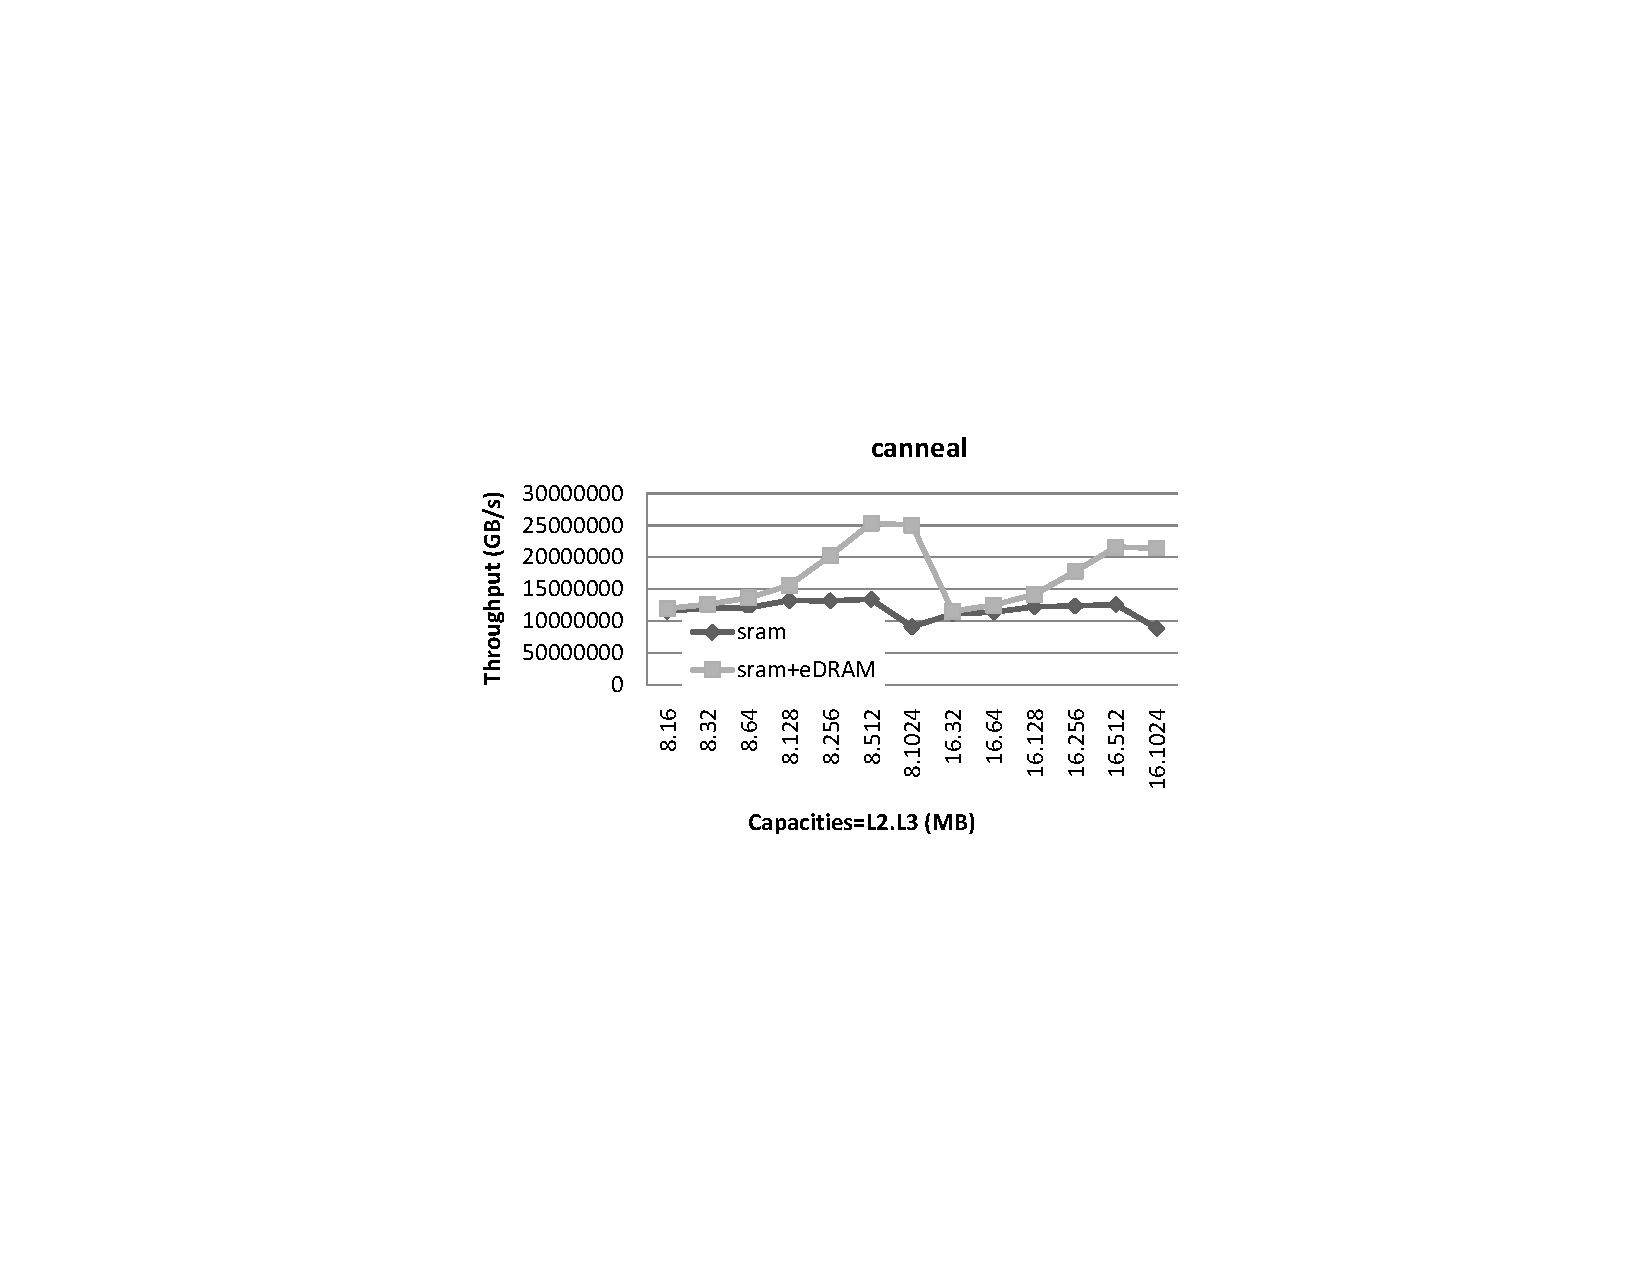
\includegraphics[width=2.5in]{figures/canneal-l2l3}\hspace{0.2in}
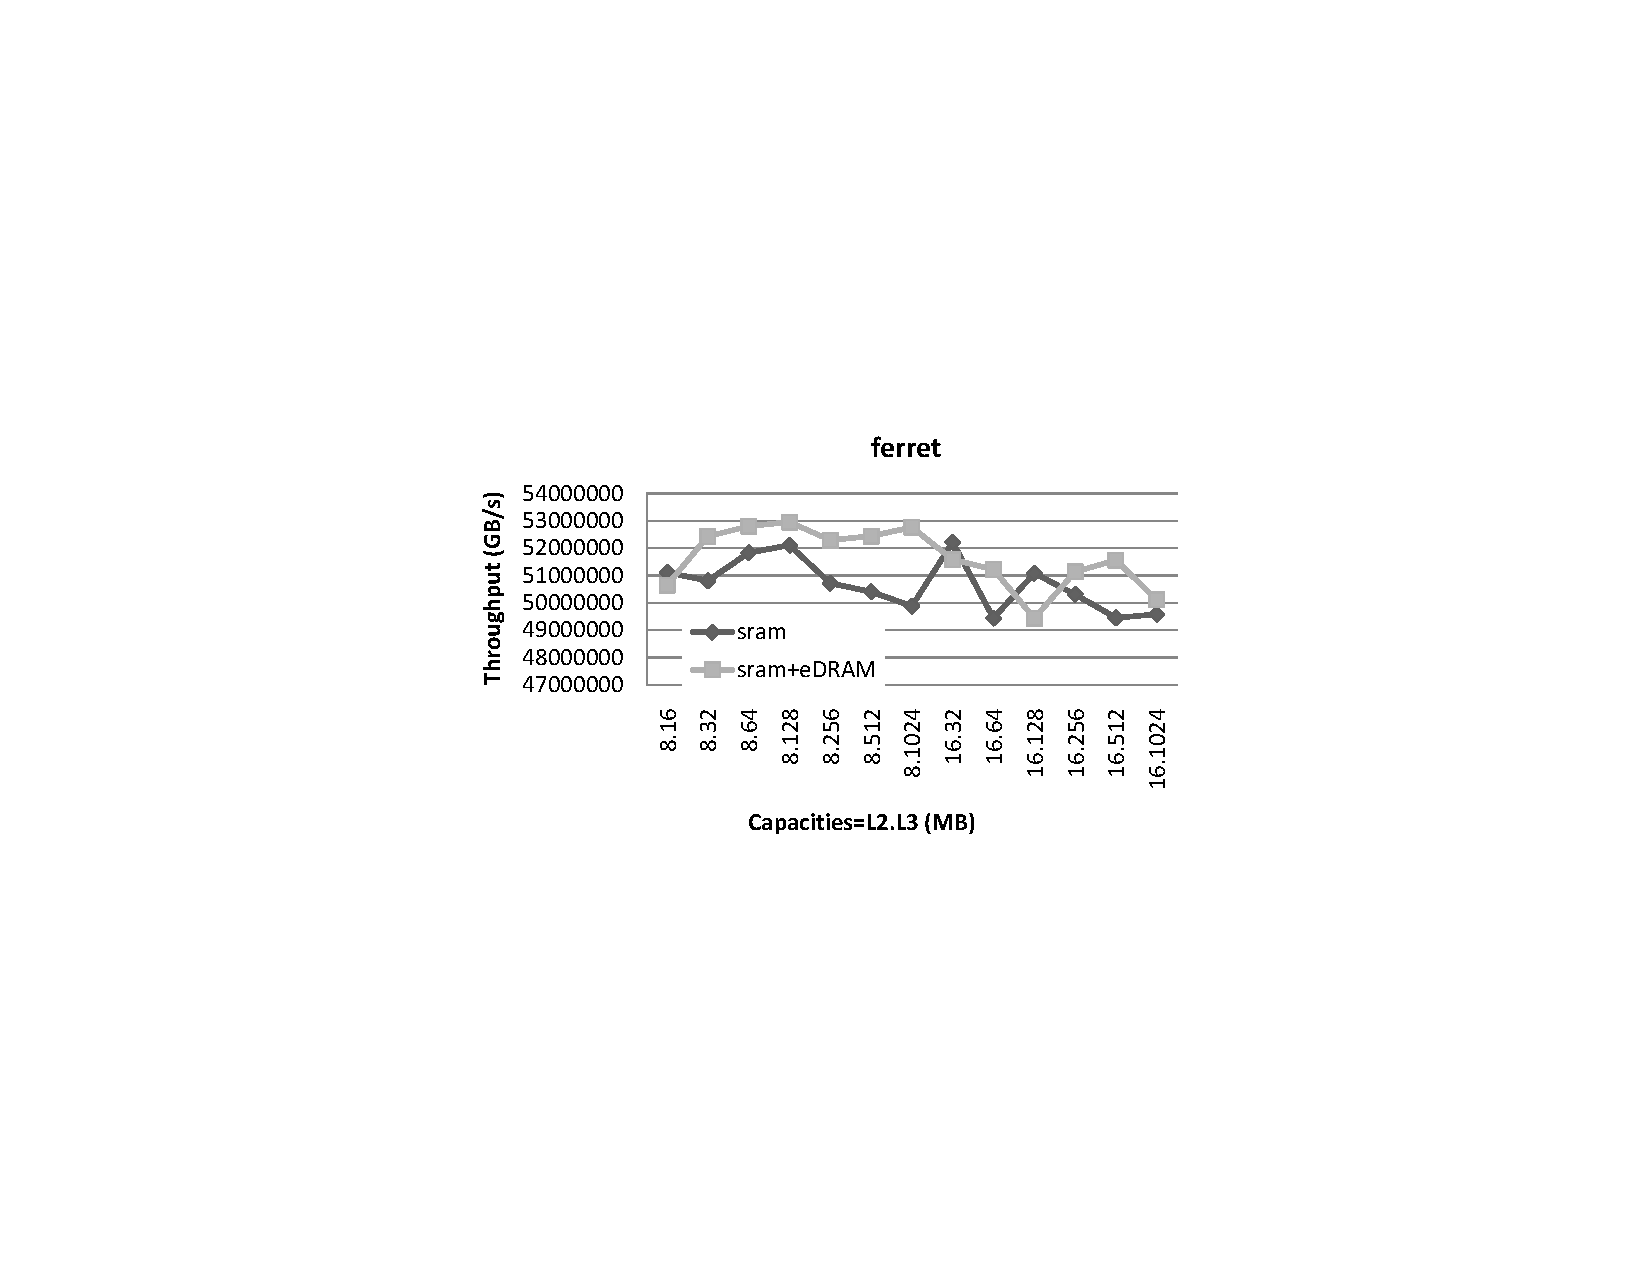
\includegraphics[width=2.5in]{figures/ferret-l2l3}\\
\hspace{0.02in}
\makebox[2.5in][l]{\bf (a)}
\makebox[2.5in][l]{\bf (b)}
\caption{Performance comparison with two-level caches among various cache
  capacity. (a) The canneal benchmark. (b) The ferret benchmark.}
\label{fig:benchmark-l2l3}
\end{figure*}

In the second set of experiments, we evaluate the system performance with
three-level shared caches. When evaluating hybrid cache configurations, we
consider implementing the last level cache by MRAM and RRAM memory technologies,
since the data transaction intensity is relatively low in the last level cache.
Figure~\ref{fig:thput-l2l3l4} shows the results.
Figure~\ref{fig:thput-l2l3l4}(a) illustrated that the performance more than 15\%
higher on average with a last level cache implemented by MRAM than pure SRAM
implementations. More performance improvement is obtained by increasing the last
level cache capacity, as shown in Figure~\ref{fig:thput-l2l3l4}(b).
Figure~\ref{fig:benchmark-l2l3l4} compares performance with pure SRAM and hybrid
cache implementations with different capacities. In this case, hybrid cache
implementation leads to higher performance in both benchmarks. The results of
the two sets of experiments are illustrated together in
Figure~\ref{fig:benchmark-overall}. An interesting observation is that hybrid
cache implementation shows high performance improvement with one of the
applications \emph{canneal}, whereas as little improvement with the other
\emph{ferret}. The reason is that write latency of both MRAM and RRAM is higher
than SRAM when capacity is less than 1GB. Performance of applications with large
number of writes, such as \emph{ferret} is therefore not benefit from hybrid
cache design.

\begin{figure*}[t]
\centering
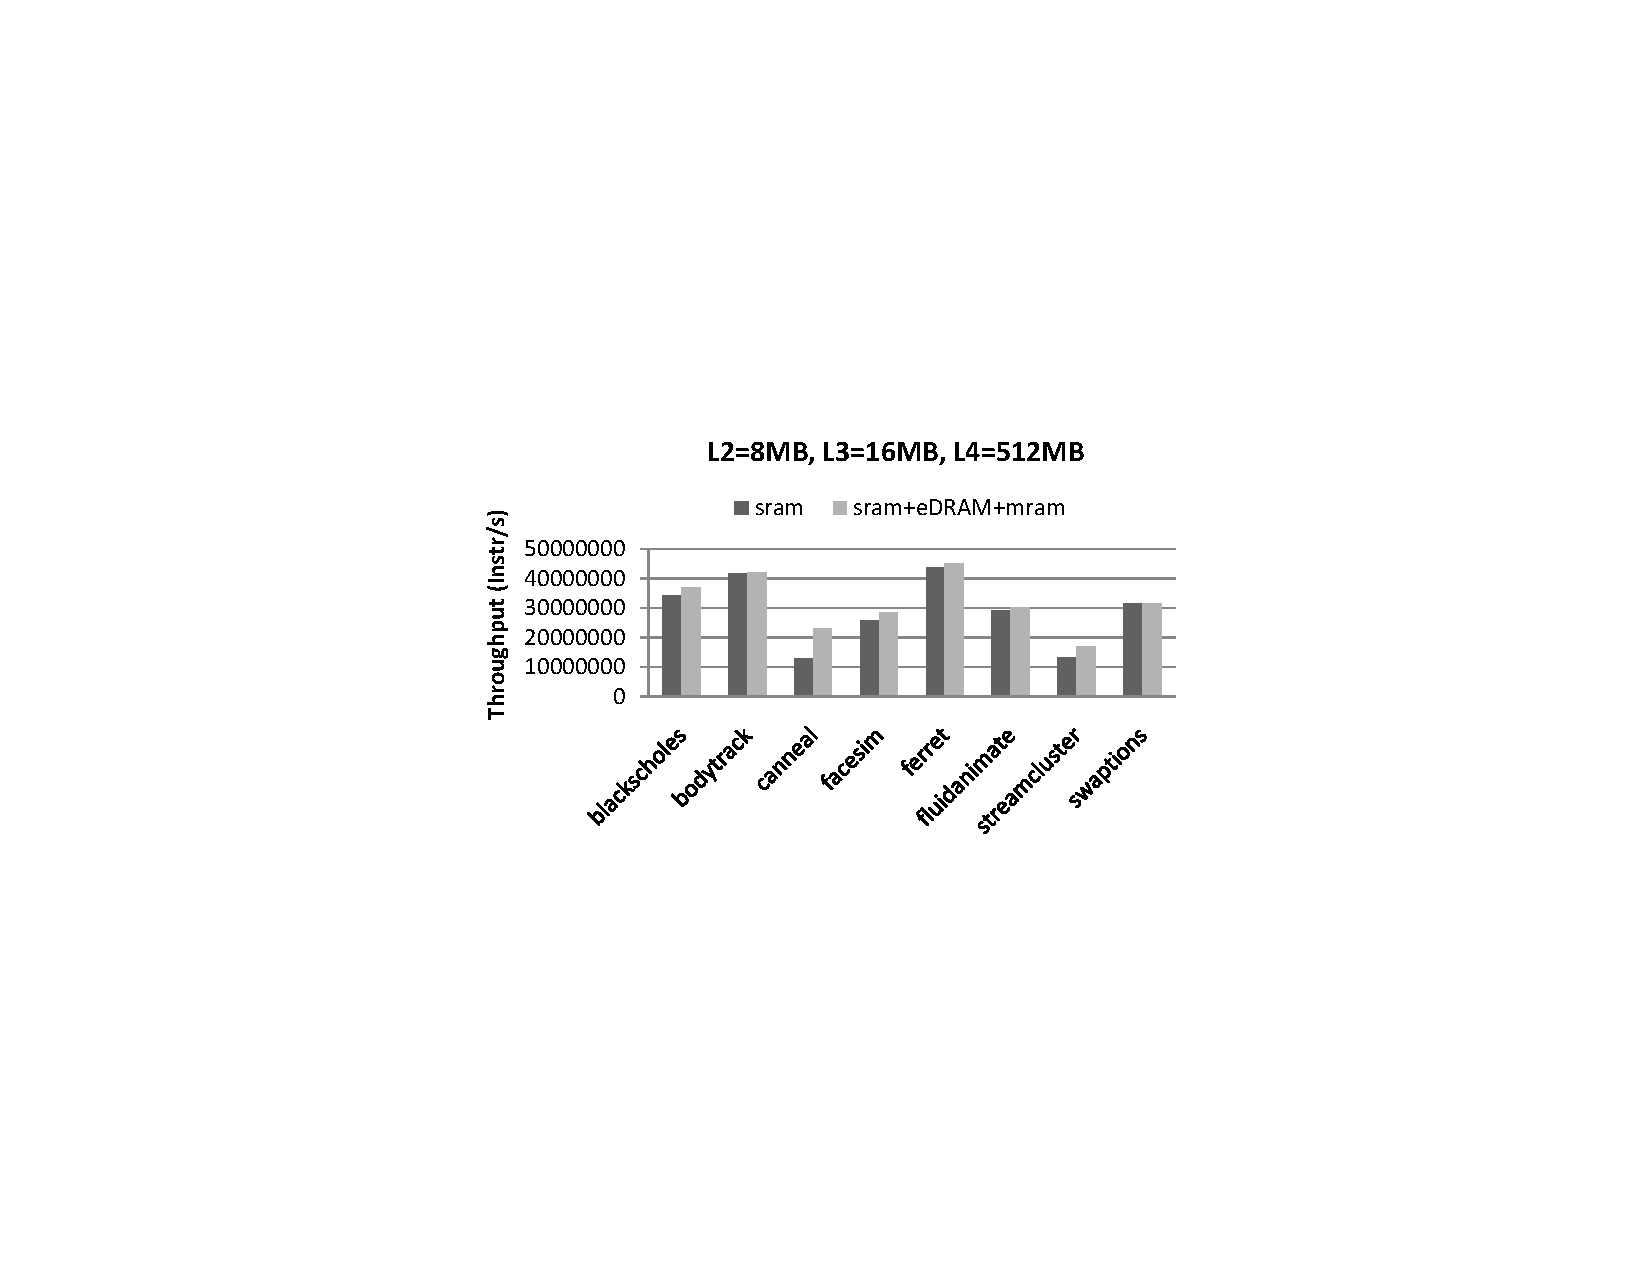
\includegraphics[width=2.5in]{figures/thput-l2l3l4-1}\hspace{0.2in}
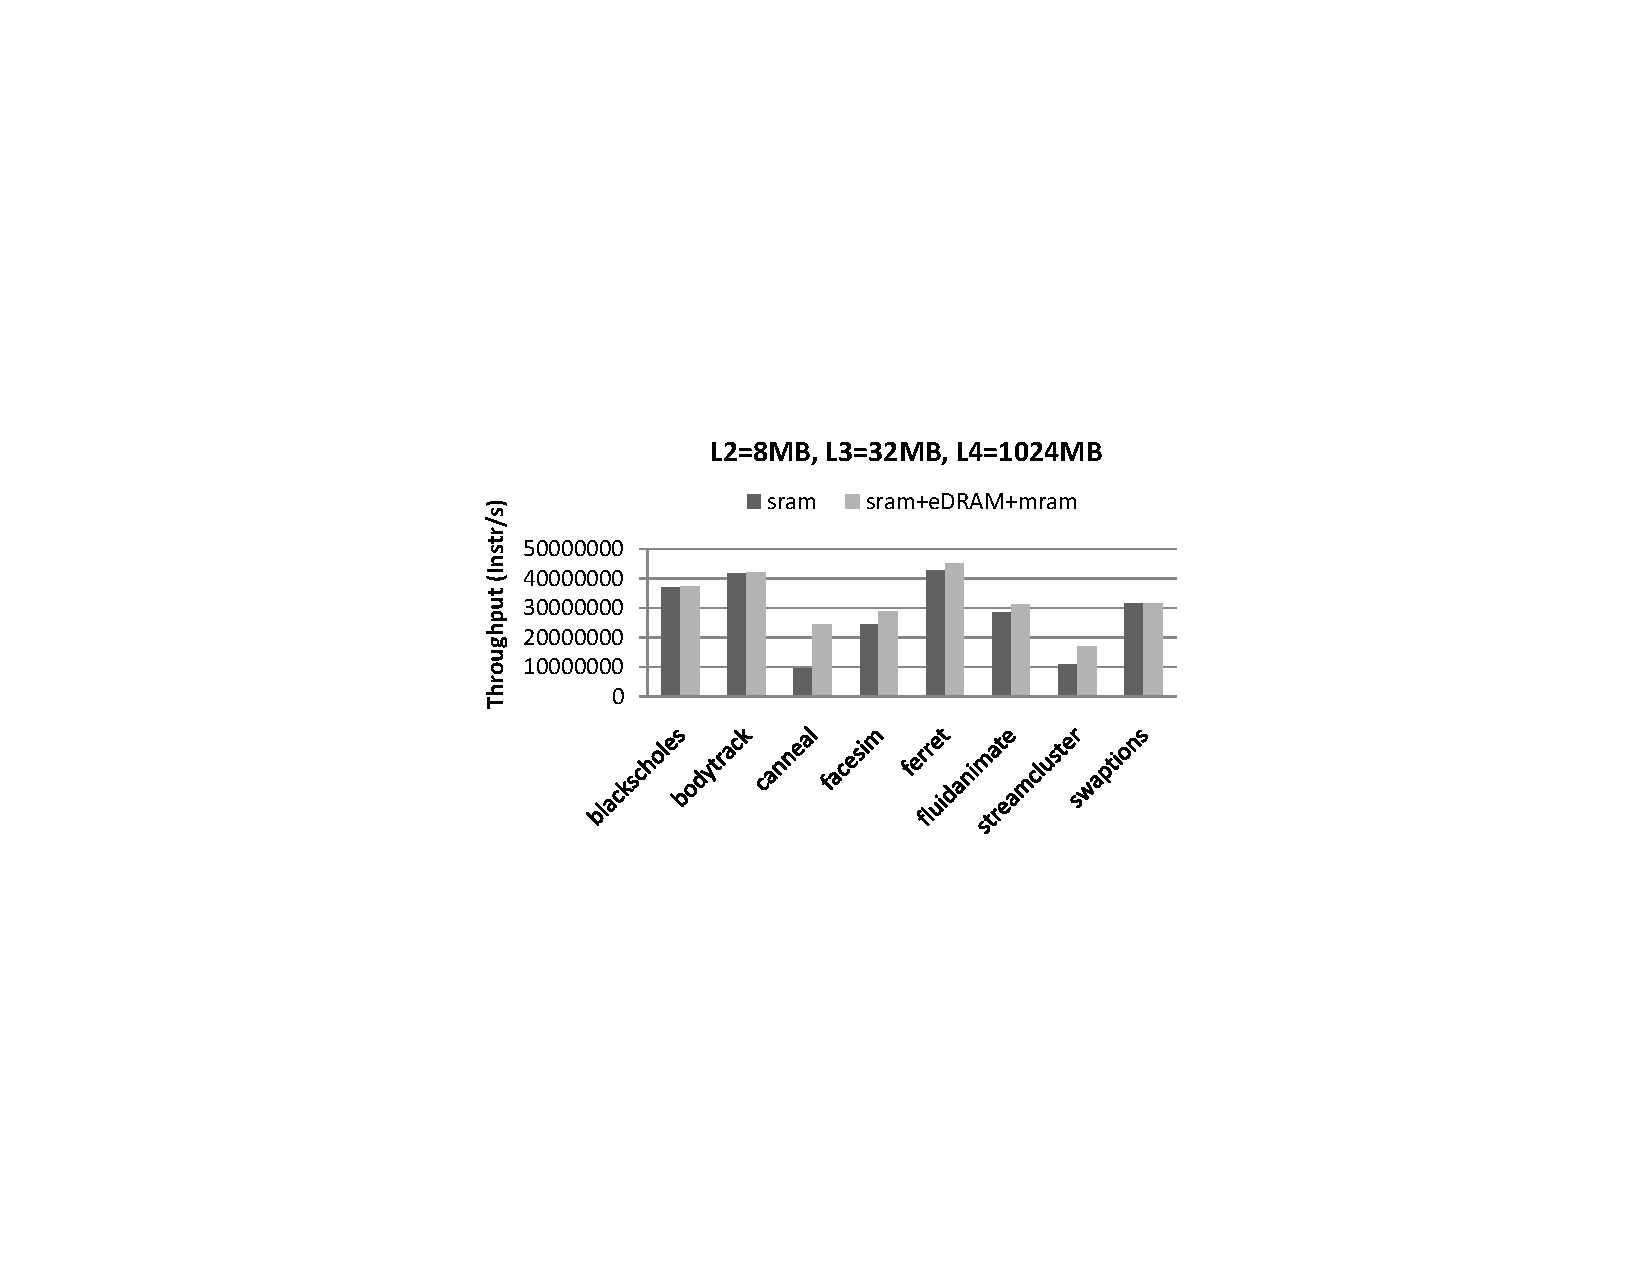
\includegraphics[width=2.5in]{figures/thput-l2l3l4-2}\\
\hspace{0.02in}
\makebox[2.5in][l]{\bf (a)}
\makebox[2.5in][l]{\bf (b)}

\caption{Performance comparison with three-level caches among various
  benchmarks. (a) The L3 cache capacity is 16MB, and the L4 cache capacity is
  512MB. (b) The L3 cache capacity is 32MB, and the L4 cache capacity is 1GB.}
\label{fig:thput-l2l3l4}
\end{figure*}

\begin{figure*}[t]
\centering
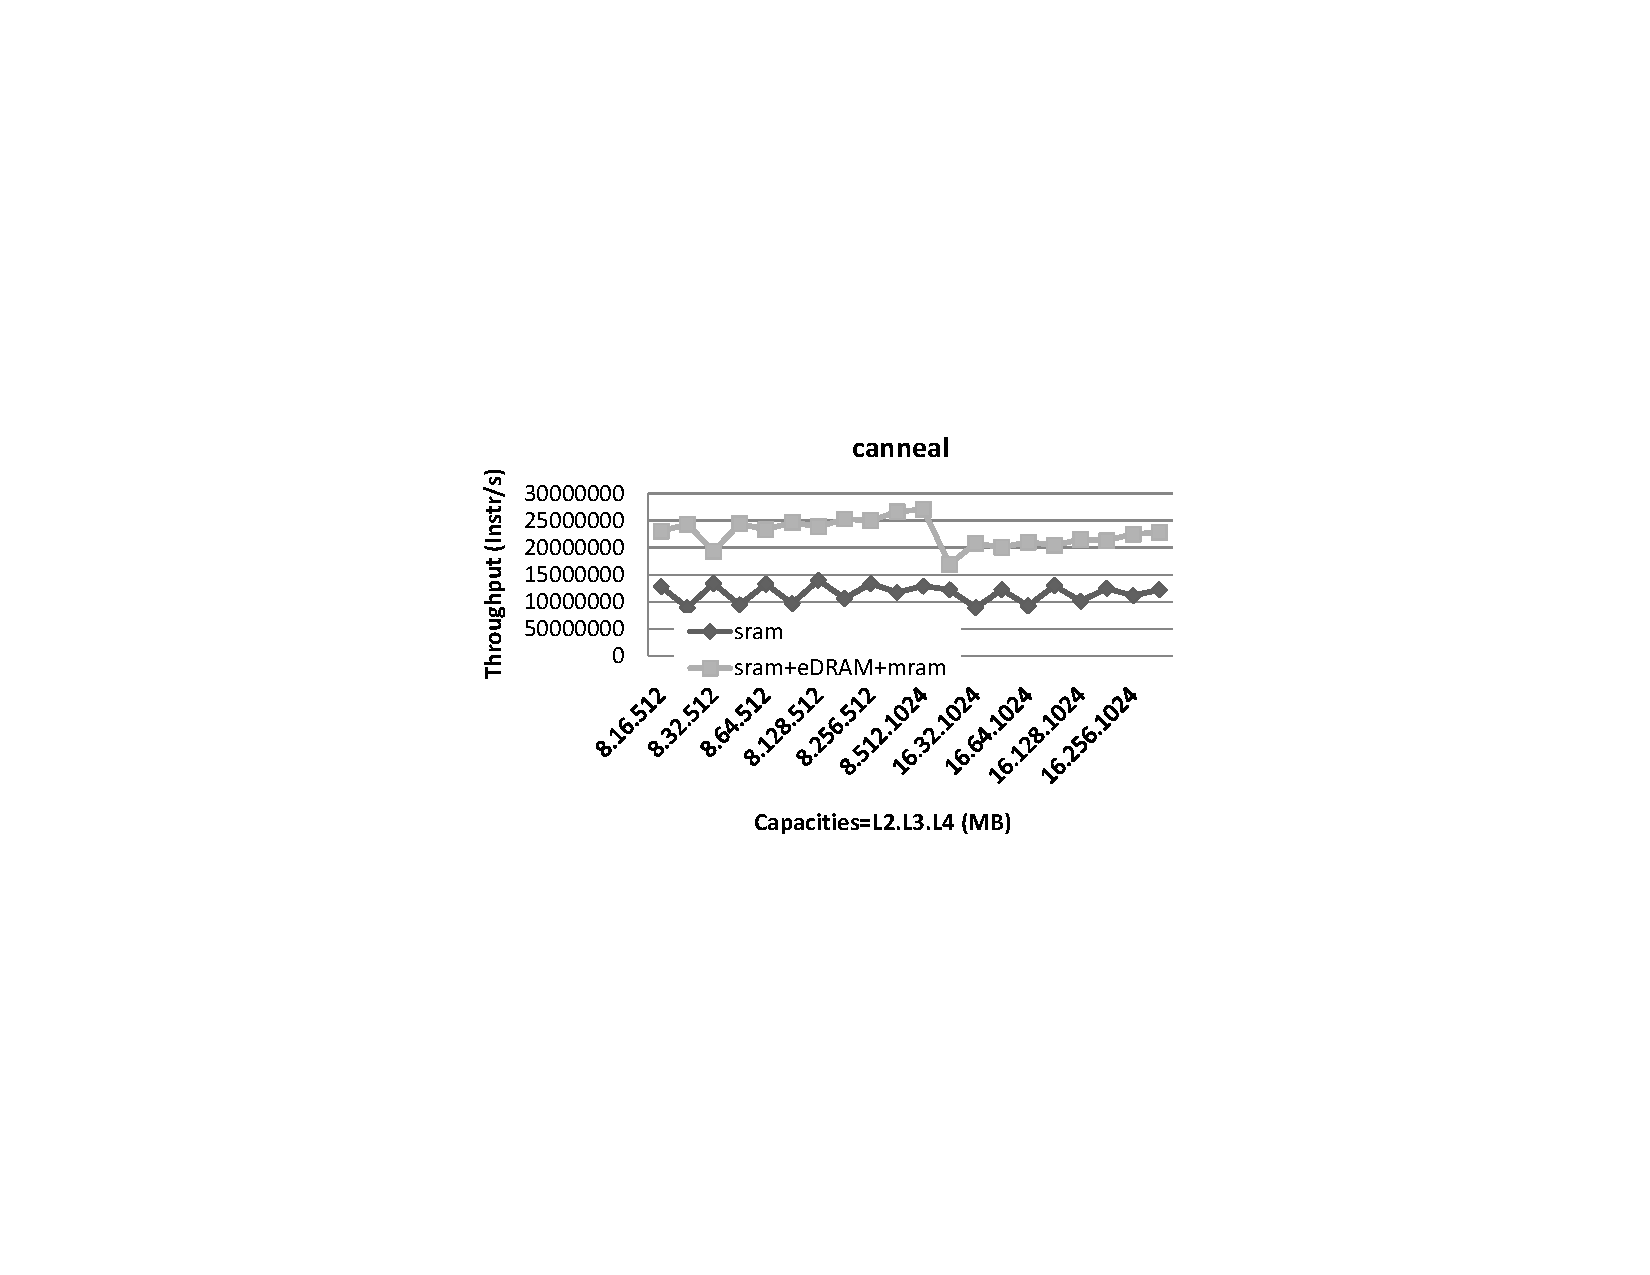
\includegraphics[width=2.5in]{figures/canneal-l2l3l4}\hspace{0.2in}
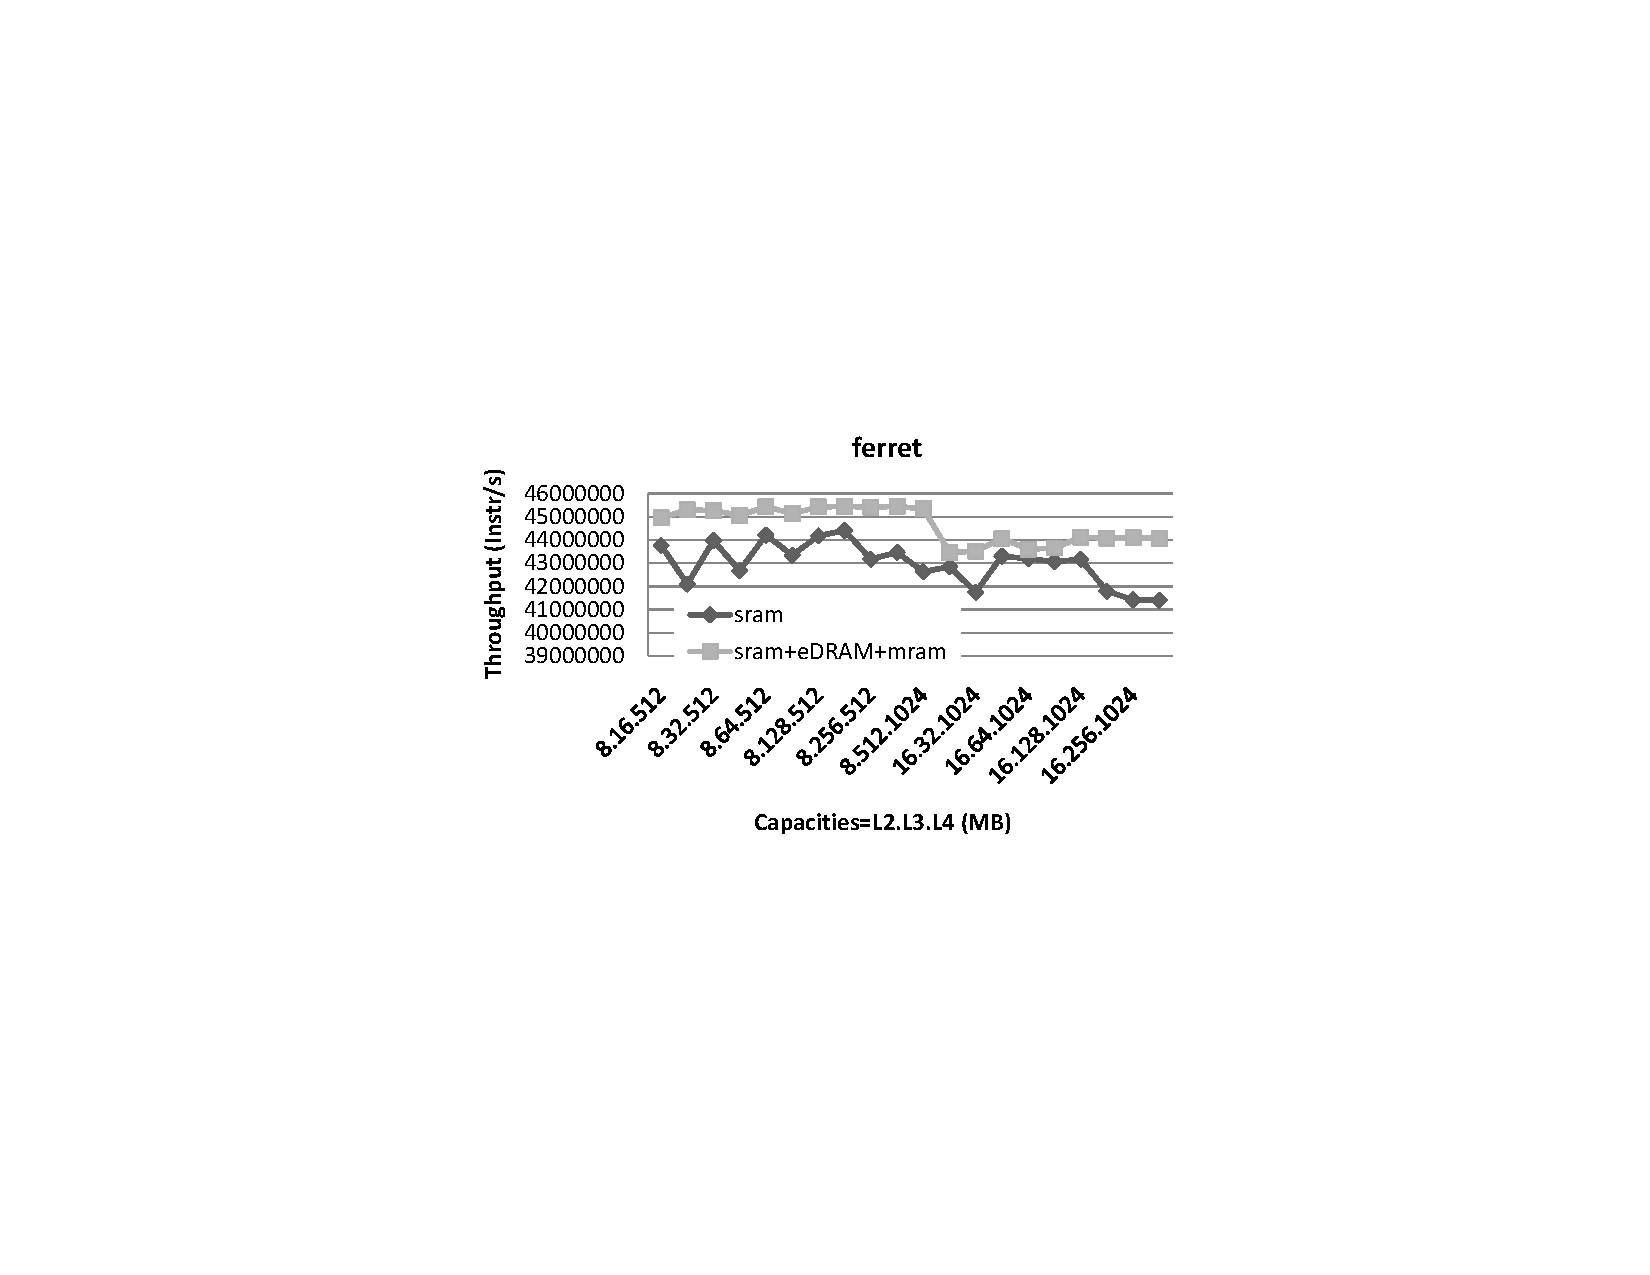
\includegraphics[width=2.5in]{figures/ferret-l2l3l4}\\
\hspace{0.02in}
\makebox[2.5in][l]{\bf (a)}
\makebox[2.5in][l]{\bf (b)}
\caption{Performance comparison with three-level caches among various cache
  capacity. (a) The canneal benchmark. (b) The ferret benchmark..}
\label{fig:benchmark-l2l3l4}
\end{figure*}

\begin{figure*}[t]
\centering
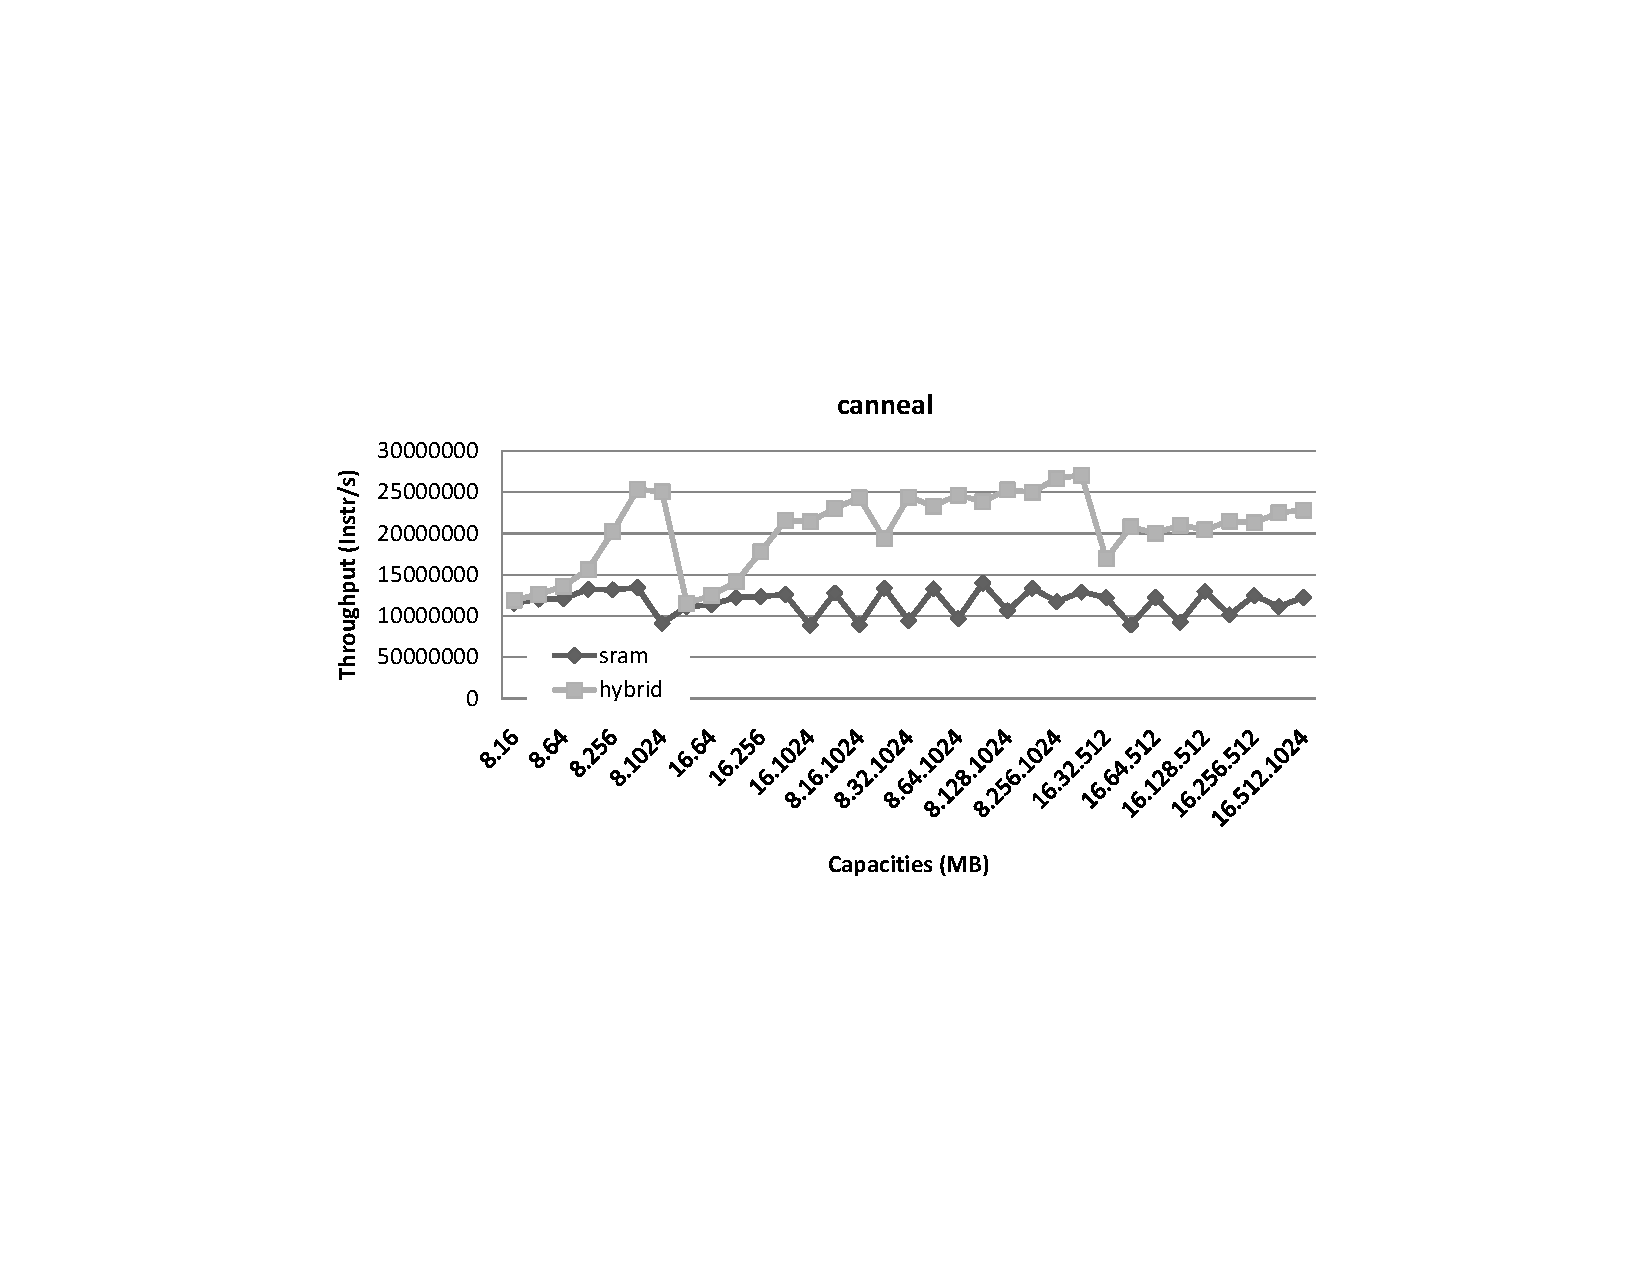
\includegraphics[width=2.5in]{figures/canneal}\hspace{0.2in}
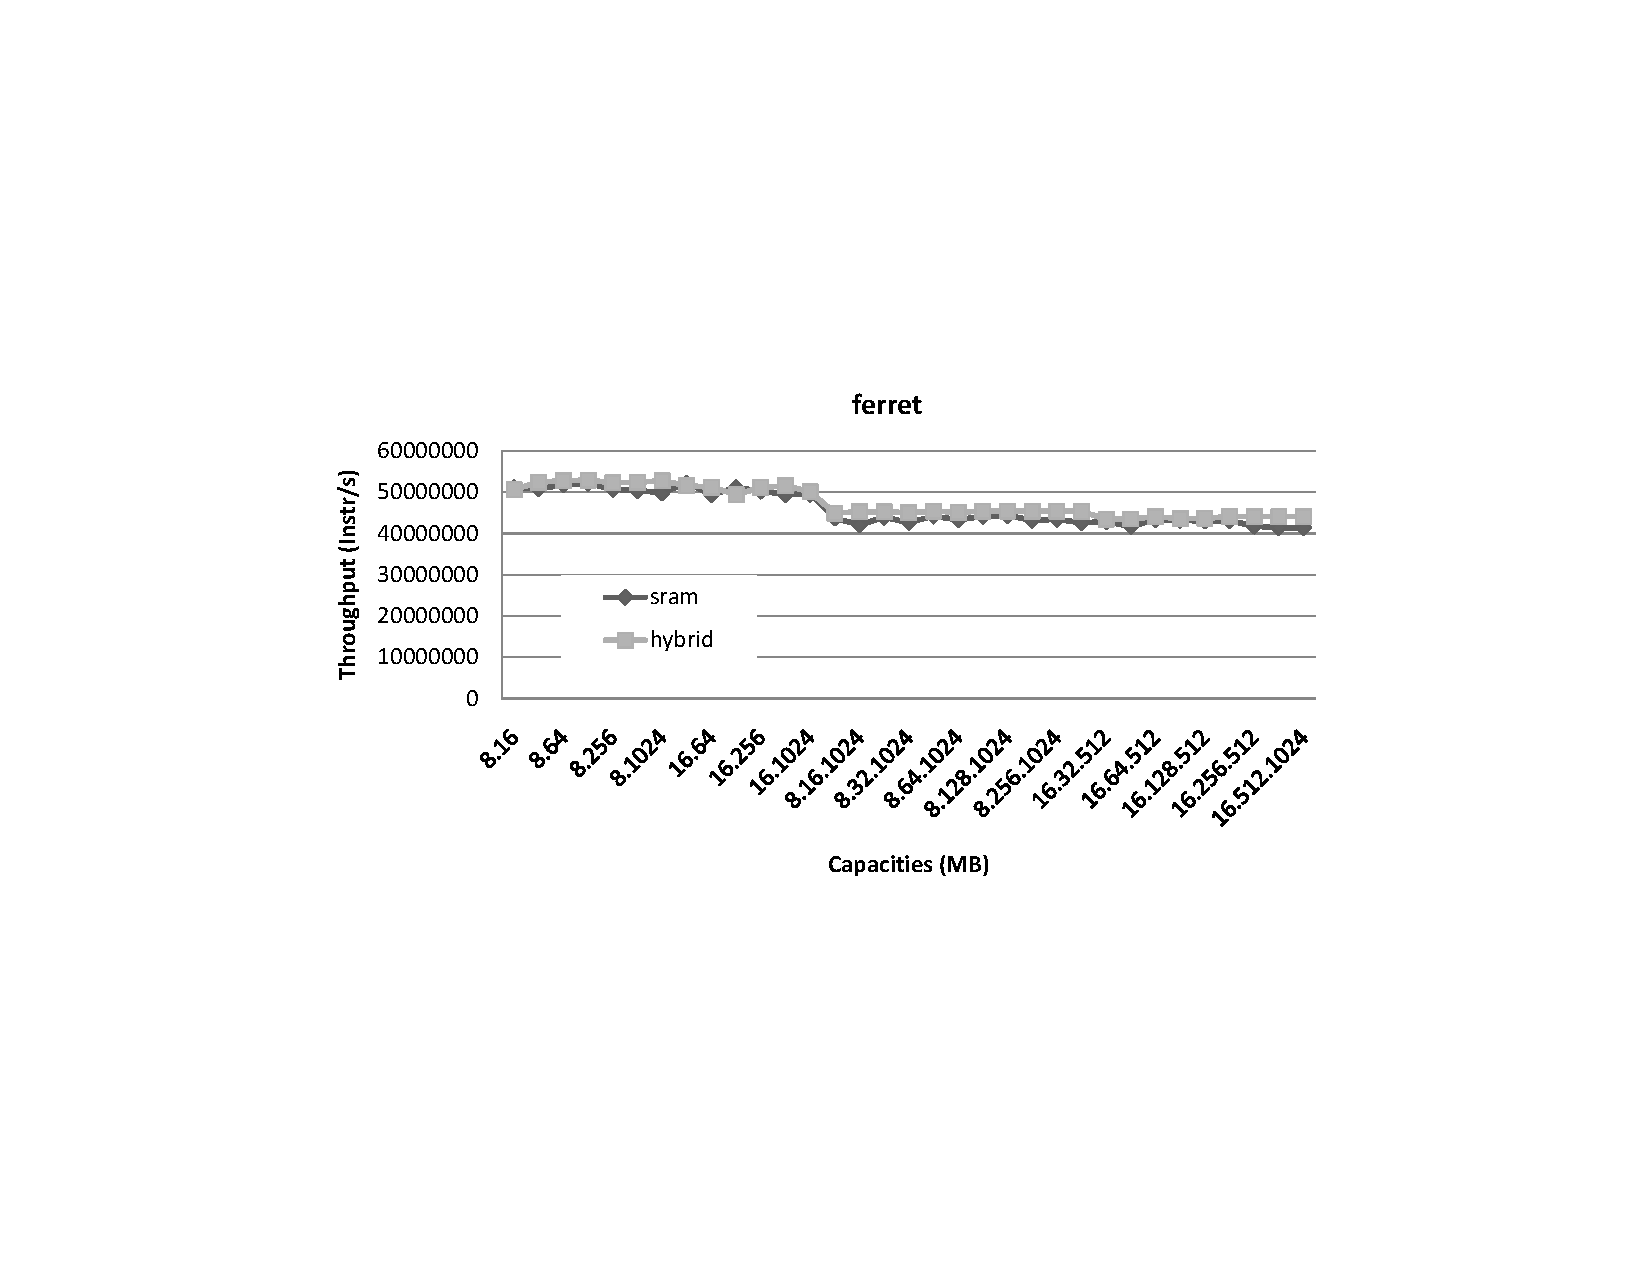
\includegraphics[width=2.5in]{figures/ferret}\\
\hspace{0.02in}
\makebox[2.5in][l]{\bf (a)}
\makebox[2.5in][l]{\bf (b)}

\caption{Performance comparison with both two-level and three-level caches among
  various cache capacity. (a) The canneal benchmark. (b) The ferret benchmark.}
\label{fig:benchmark-overall}
\end{figure*}

Finally, we evaluate all the possible cache hierarchy configurations with
exhaustive simulations. The optimal cache configurations of each benchmark is
shown in Table~\ref{table:results}. Since the characteristics vary among the
benchmarks, the optimal cache configurations are different among each of
benchmarks. Applications with high write intensities, such as \emph{bodytrack},
\emph{ferret}, and \emph{swaptions} tend to favor SRAM-based caches. Other
applications benefit more from hybrid cache implementation in terms of
performance.

\begin{table*}[t]
  \centering
  \caption{Optimal cache configurations for each benchmark.}
  \vspace{0.1in}
  \begin{tabular}{l|c|c|c}
    \hline\hline
    \textbf{Benchmarks} & \textbf{L2} & \textbf{L3} & \textbf{L4}\\
    \hline
    blackscholes & SRAM, 8MB & eDRAM, 32MB & RRAM, 1GB\\
    \hline
    bodytrack & SRAM, 8MB & eDRAM, 128MB & -\\
    \hline
    canneal & SRAM, 8MB & eDRAM, 512MB & MRAM, 1GB\\
    \hline
    facesim & SRAM, 8MB & eDRAM, 32MB & MRAM, 1GB\\
    \hline
    ferret & SRAM, 8MB & eDRAM, 32MB & -\\
    \hline
    fluidanimate & SRAM, 8MB & eDRAM, 1GB & -\\
    \hline
    streamcluster & SRAM, 16MB & eDRAM, 128MB & MRAM, 512MB\\
    \hline
    swaptions & SRAM, 8MB & SRAM, 32MB & SRAM, 1GB\\
    \hline\hline
  \end{tabular}
  \label{table:results}
\end{table*}

% --------------------------------------------------------------------------
\section{Conclusion and Future Work}
In this project, we explore performance and energy characteristics of various
emerging memory technolgies. Based on our exploration, we evaluate the shared
cache hierarchy design of CMPs optimized for performance by filling the off-chip
memory bandwidth gap. According to our evaluation, SRAM-based caches leads to
reasonable performance with write-intensive applications. Hybrid cache design
help with performance with other types of benchmarks.

Furthermore, a variety of continuing studies is remained to be explored related
to bandwidth-aware memory hierarchy design. First of all, we only examine cache
hierarchy design currently. It is necessary to extend our exploration to the
overall memory hierarchy design. On the other hand, we do not consider energy
efficiency in this project. We would like to put some power constraints to the
memory hierarchy, and examine the energy efficiency of various memory hierarchy
configurations.

\bibliographystyle{IEEEtran}
\bibliography{./bib/ref,./bib/reram,./bib/cacti}

\end{document}
